\documentclass[aspectratio=169]{beamer}
\useinnertheme{rectangles}

\definecolor{TUM-blue}{RGB}{0,101,189}
\usecolortheme[named=TUM-blue]{structure}

\setbeamertemplate{navigation symbols}{%
    \usebeamerfont{footline}%
    \usebeamercolor[fg]{footline}%
    \hspace{1em}%
    \insertframenumber/\inserttotalframenumber
}
\setbeamercolor{footline}{fg=black}
\setbeamerfont{footline}{series=\bfseries}

\usepackage[justification=centering, font=footnotesize]{caption}
\usepackage{braket}
\usepackage{etoolbox}
\usepackage{expl3}
\usepackage{animate}
\usepackage{graphicx}
\usepackage{mathtools}
\usepackage{amsmath}
\usepackage{amssymb}
% \usepackage{multirow}

\title{Quantum Cellular Automata}
\subtitle{The Quantum Game of Life}

\author{Benjamin Decker}
\institute[]{Technical University of Munich}
\date{9. June 2022}

\newcommand{\hamiltonianPaper}{\hat{H}=\sum_{i=3}^{L - 2}\hat{S}_i\left(\hat{N}_i^{(2)} + \hat{N}_i^{(3)}\right)}
\newcommand{\unitary}{\hat{U}(t)=e^{-\mathrm{i}\hat{H}t}}
\newcommand{\timeEvolution}{\ket{\psi}_t=\hat{U}(t)\ket{\psi}_0}
\newcommand{\timeStepEvolution}{\ket{\psi}_k=\left(\hat{U}\left(\frac{\pi}{2}\right)\right)^k\ket{\psi}_0}
\newcommand{\singleTimeStepEvolution}{\ket{\psi}_{k+1}=\hat{U}\left(\frac{\pi}{2}\right)\ket{\psi}_k}
\newcommand{\variableSingleTimeStepEvolution}{\ket{\psi}_{k+1}=\hat{U}\left(t\right)\ket{\psi}_k}
\newcommand{\hamiltonianGeneral}{\hat{H}=\sum_{i}\hat{S}_i\left(\hat{N}_i\right)}
\newcommand{\vonNeumannEntropy}{S(\rho_A) = -Tr(\rho_Alog_2(\rho_A))}
\newcommand{\projdown}{\hat{\bar{n}}}
\newcommand{\projup}{\hat{n}}

\ExplSyntaxOn
\newcommand{\helper}[1]{
    \str_case:nnF {#1}{
        {0} {\projdown}
        {1} {\projup}
    }{\PackageError{a}{a}{a}}
}
\ExplSyntaxOff
\newcommand{\makesummand}[4]{
    \helper{#1}_{i-2}\helper{#2}_{i-1}\helper{#3}_{i+1}\helper{#4}_{i+2}
}

\begin{document}

\begin{frame}
\begin{columns}
\column{.5\textwidth}
\titlepage
\column{.5\textwidth}
\begin{figure}
    \centering
    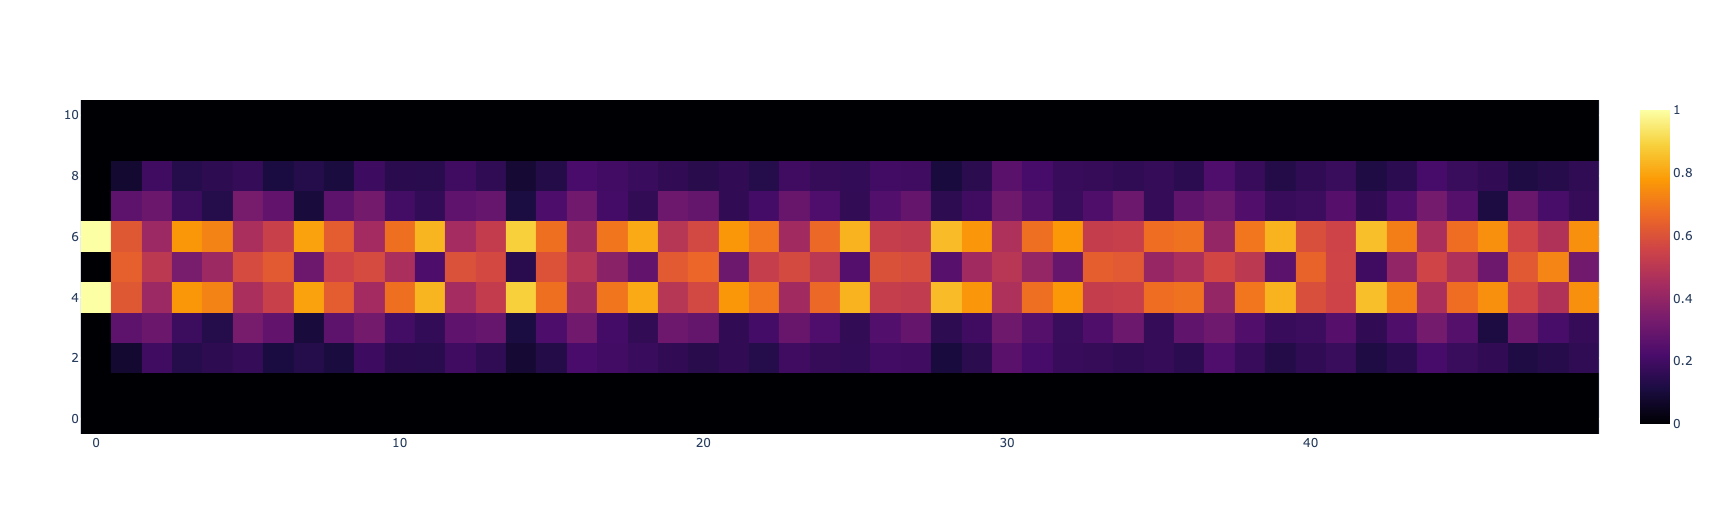
\includegraphics[width=\columnwidth]{graphics/blinker.png}
    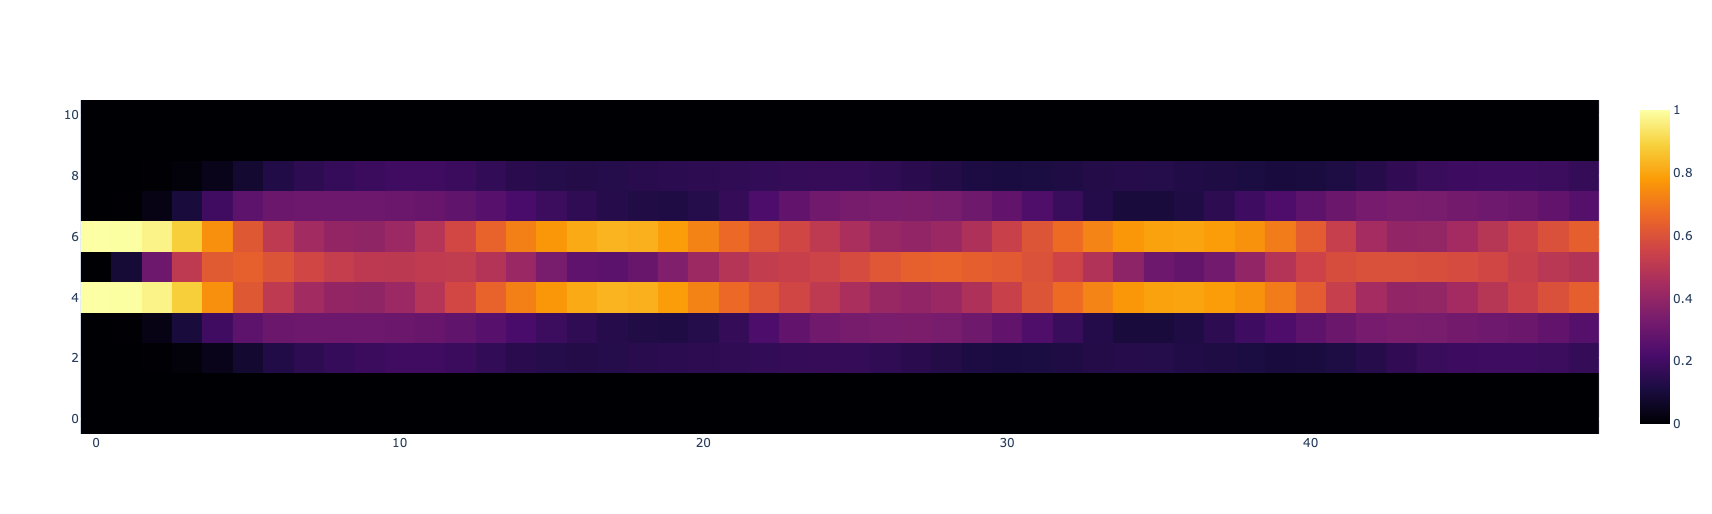
\includegraphics[width=\columnwidth]{graphics/blinker_slow.png}
    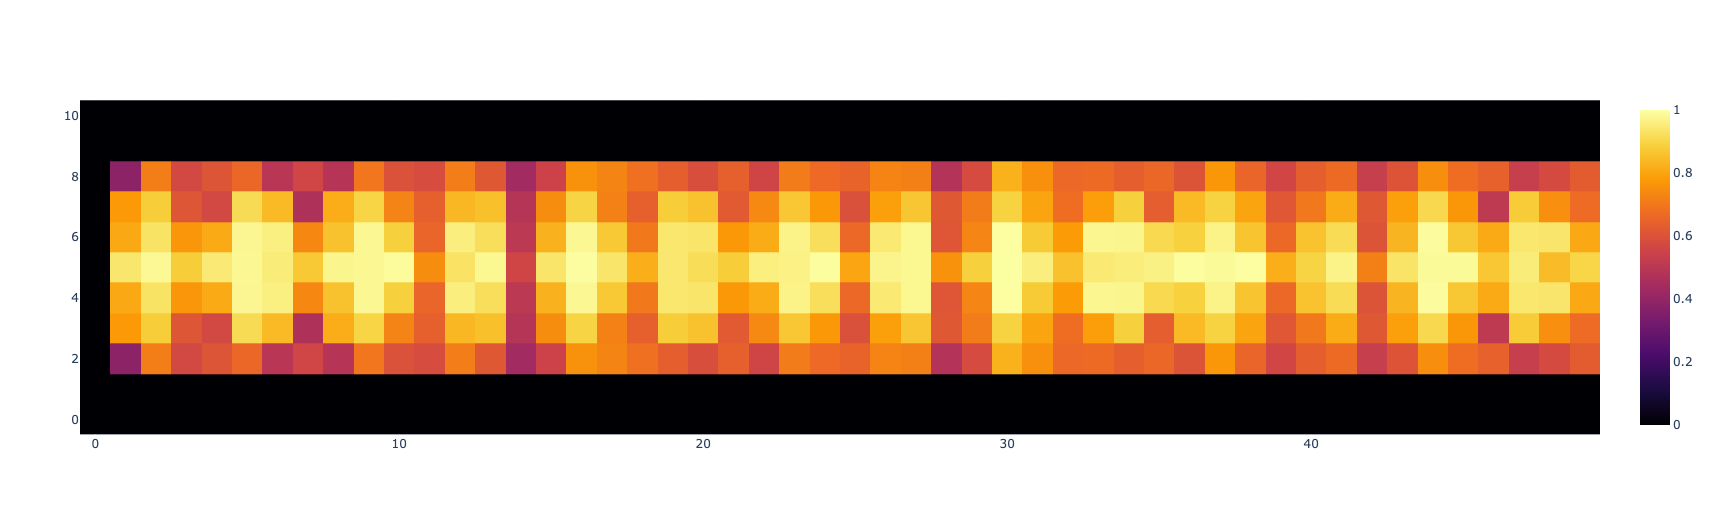
\includegraphics[width=\columnwidth]{graphics/blinker_sse.png}
\end{figure}
\end{columns}
\end{frame}

\begin{frame}[t]{Classical Cellular Automata}
    \begin{itemize}
        \item Grid of cells in one or more dimensions evolving over time steps
        \item State in time step $t+1$ depends only on state in time step $t$
    \end{itemize}
    \begin{columns}
    \column{.4\textwidth}
    \begin{figure}
        \centering
        \animategraphics[
            width=\columnwidth,
            autoplay,
            loop
        ]{2}{graphics/gosper-gun/gosper-gun-}{0}{29}
        \caption{Gosper's glider gun from Conway's Game of Life}
        \label{fig:conway}
    \end{figure}
    \column{.6\textwidth}
    \begin{figure}
        \centering
        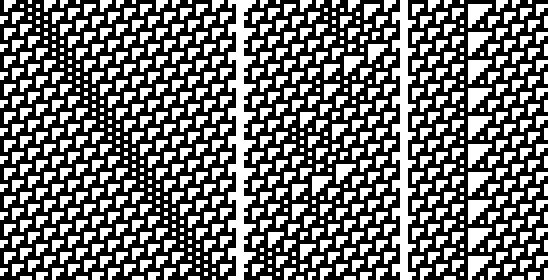
\includegraphics[width=\columnwidth]{graphics/R110.png}
        \caption{A glider in the rule-110 elementary cellular automaton}
        \label{fig:my_label}
    \end{figure}
    \end{columns}
    \vspace{1000pt}
\end{frame}

\begin{frame}[t]{What do we need?}
    \begin{itemize}
        \onslide<2->{
        \item Represent a classical state with a quantum state \ \onslide<4->{{\tiny$010\Longrightarrow\ket{\psi}=\ket{0}\otimes\ket{1}\otimes\ket{0}$}}
        }
        \only<5->{
        \item Extract the distribution of alive cells from the quantum state \ \onslide<7->{{\tiny$P(alive)_j=\bra{\psi}\projup_j\ket{\psi}$}}
        }
        \only<8->{
        \item Let $\ket{\psi}$ evolve with time according to the rules of the QCA
        }
    \end{itemize}
    \only<3>{
    \vspace{15pt}
    \begin{columns}
    \column{.5\textwidth}
        \begin{center}
            $0\coloneqq dead$
        \end{center}
        \begin{center}
            $\ket{0}\coloneqq 0$
        \end{center}
    \column{.5\textwidth}
        \begin{center}
            $1\coloneqq alive$
        \end{center}
        \begin{center}
            $\ket{1}\coloneqq 1$
        \end{center}
    \end{columns}
    \begin{center}
        $000101000\Longrightarrow\ket{\psi}=\ket{0}^{\otimes3}\otimes\ket{1}\otimes\ket{0}\otimes\ket{1}\otimes\ket{0}^{\otimes3}$
    \end{center}
    }
    \only<6>{
    \vspace{15pt}
    \begin{center}
        To compute the probability that cell $j$ is alive or dead, we measure with the corresponding observable
    \end{center}
    \begin{columns}
    \column{.5\textwidth}
    \begin{center}
        $\projdown_j = \ket{0}_j\bra{0}$
    \end{center}
    \column{.5\textwidth}
    \begin{center}
        $\projup_j = \ket{1}_j\bra{1}$
    \end{center}
    \end{columns}
    \begin{columns}
    \column{.5\textwidth}
    \begin{center}
        $P(dead)_j=\bra{\psi}\projdown_j\ket{\psi}$
    \end{center}
    \column{.5\textwidth}
    \begin{center}
        $P(alive)_j=\bra{\psi}\projup_j\ket{\psi}$
    \end{center}
    \end{columns}
    }
    \only<9->{
    \vspace{15pt}
    \begin{center}
        For an initial state $\ket{\psi}_0$ and the unitary time evolution operator $\hat{U}(k)$, the state after $k$ time steps is given by
    \end{center}
    \vspace{10pt}
    \begin{equation*}
        \ket{\psi}_k=\hat{U}(k)\ket{\psi}_0
    \end{equation*}
    }
    \only<10->{
    \vspace{2pt}
    \begin{center}
        How do we get $\hat{U}(k)$?
    \end{center}
    }
    \vspace{1000pt}
\end{frame}

\begin{frame}[t]{Hamiltonian}
    \begin{equation}
        \hamiltonianPaper
        \label{eq:hamiltonianPaper}
    \end{equation}
    \only<2-4>{
    \vspace{10pt}
    \begin{center}
        Rule $F_{12}$:\\"A cell is flipped if the number of alive cells among its nearest and next-nearest neighbors is $2$ or $3$"
    \end{center}
    }
    \only<3-4,6-7>{
    \vspace{10pt}
    \begin{itemize}
    \onslide<3->{
    \item Operator $\hat{S}_i$ flips the $i$-th cell, i.e. $\hat{S}_i = (\sigma_x)_i$
    }
    \onslide<4->{
    \item Operators $\hat{N}_i$ are chosen to be non-zero over the set of states where the rule applies
    }
    \onslide<7->{
    \item As visible from the summation index $i$, constant boundary conditions are used
    }
    \end{itemize}
    }
    \only<5>{
    \vspace{15pt}
    \begin{columns}
    \column{.5\textwidth}
    \begin{center}
        $\projdown_j = \ket{0}_j\bra{0}$
    \end{center}
    \column{.5\textwidth}
    \begin{center}
        $\projup_j = \ket{1}_j\bra{1}$
    \end{center}
    \end{columns}
    
    \begin{equation*}
        \begin{split}
        \hat{N}_i^{(2)}=\ &\makesummand{0}{0}{1}{1}+\makesummand{0}{1}{0}{1}\\
        +\ &\makesummand{0}{1}{1}{0}+\makesummand{1}{0}{0}{1}\\
        +\ &\makesummand{1}{0}{1}{0}+\makesummand{1}{1}{0}{0}
        \end{split}
    \end{equation*}
    \begin{equation*}
        \begin{split}
        \hat{N}_i^{(3)}=\ &\makesummand{0}{1}{1}{1}+\makesummand{1}{0}{1}{1}\\
        +\ &\makesummand{1}{1}{0}{1}+\makesummand{1}{1}{1}{0}
        \end{split}
    \end{equation*}
    }
    \onslide<8->{
    \begin{center}
        By solving the Schrödinger equation $$\mathrm{i}\partial_t\ket{\psi}_t=\hat{H}\ket{\psi}_t$$ the time evolution operator $\hat{U}$ is given by
    \end{center}
    \vspace{10pt}
    \begin{equation}
        \unitary
        \label{eq:unitary}
    \end{equation}
    }
    \vspace{1000pt}
\end{frame}

\begin{frame}[t]{Time Evolution Operator}
    \begin{equation}
        \hamiltonianPaper
        \tag{\ref{eq:hamiltonianPaper}}
    \end{equation}
    \vspace{5pt}
    \begin{equation}
        \unitary
        \tag{\ref{eq:unitary}}
    \end{equation}
    \only<2>{
    \vspace{10pt}
    \begin{center}
        For an initial state $\ket{\psi}_0$, the state after time $t$ is given by
    \end{center}
    \vspace{10pt}
    }
    \onslide<2->{
    \begin{equation}
        \timeEvolution
        \label{eq:timeEvolution}
    \end{equation}
    }
    \only<4>{
    \vspace{5pt}
    \begin{center}
        The time $t$ needed for a state to flip under the action of operator $\hat{S}_i$ is $\frac{\pi}{2}$
    \end{center}
    \begin{center}
        For a fixed time step duration $t=\frac{\pi}{2}$, the state after $k$ time steps is given by
    \end{center}
    \vspace{10pt}
    }
    \onslide<4->{
    \begin{equation}
        \timeStepEvolution
        \label{eq:timeStepEvolution}
    \end{equation}
    }
    \onslide<6->{
    \vspace{-15pt}
    \begin{center}
        \item In particular, during $1$ time step, the state of some $\ket{\psi}_k$ at time step $k$ will evolve into
    \end{center}
    \begin{equation}
        \singleTimeStepEvolution
        \label{eq:singleTimeStepEvolution}
    \end{equation}
    }
    \vspace{1000pt}
\end{frame}

\begin{frame}[t]{Iterative Calculation}
    \begin{equation}
        \singleTimeStepEvolution
        \tag{\ref{eq:singleTimeStepEvolution}}
    \end{equation}
    \only<2>{
    \begin{figure}
        \centering
        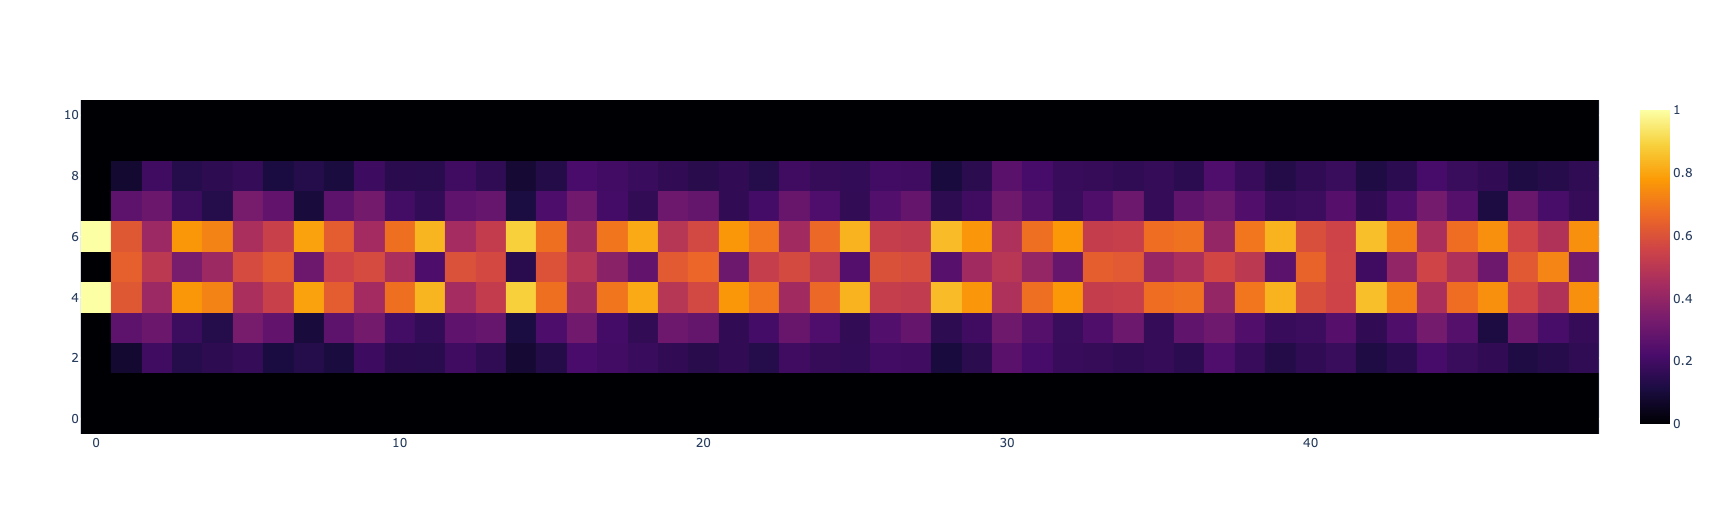
\includegraphics[width=\textwidth]{graphics/blinker.png}
        \caption{Time evolution of the initial state $\ket{\psi}_0=\ket{0}^{\otimes4}\otimes\ket{101}\otimes\ket{0}^{\otimes4}$ according to equation (\ref{eq:singleTimeStepEvolution}) shown as the distribution of alive cells}
        \label{fig:blinker}
    \end{figure}
    }
    \only<3>{
    \begin{figure}
        \centering
        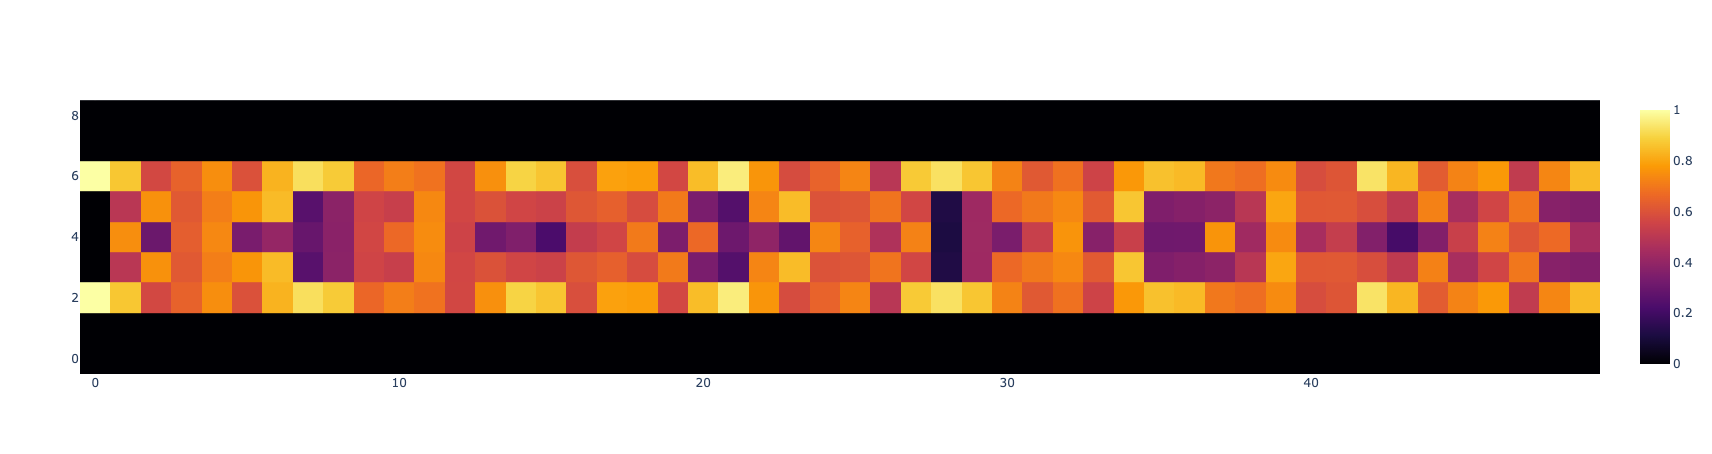
\includegraphics[width=\textwidth]{graphics/wide_blinker.png}
        \caption{Time evolution of the initial state $\ket{\psi}_0=\ket{001000100}$ according to equation (\ref{eq:singleTimeStepEvolution}) shown as the distribution of alive cells}
        \label{fig:blinker}
    \end{figure}
    }
    \vspace{1000pt}
\end{frame}

\begin{frame}[t]{Variable Time Steps}
    \only<1>{
    \begin{equation}
        \singleTimeStepEvolution
        \tag{\ref{eq:singleTimeStepEvolution}}
    \end{equation}
    }
    \onslide<2->{
    \begin{equation}
        \variableSingleTimeStepEvolution
        \label{eq:variableSingleTimeStepEvolution}
    \end{equation}
    }
    \onslide<3>{
    \begin{figure}
    \begin{columns}
    \column{.5\textwidth}
        \centering
        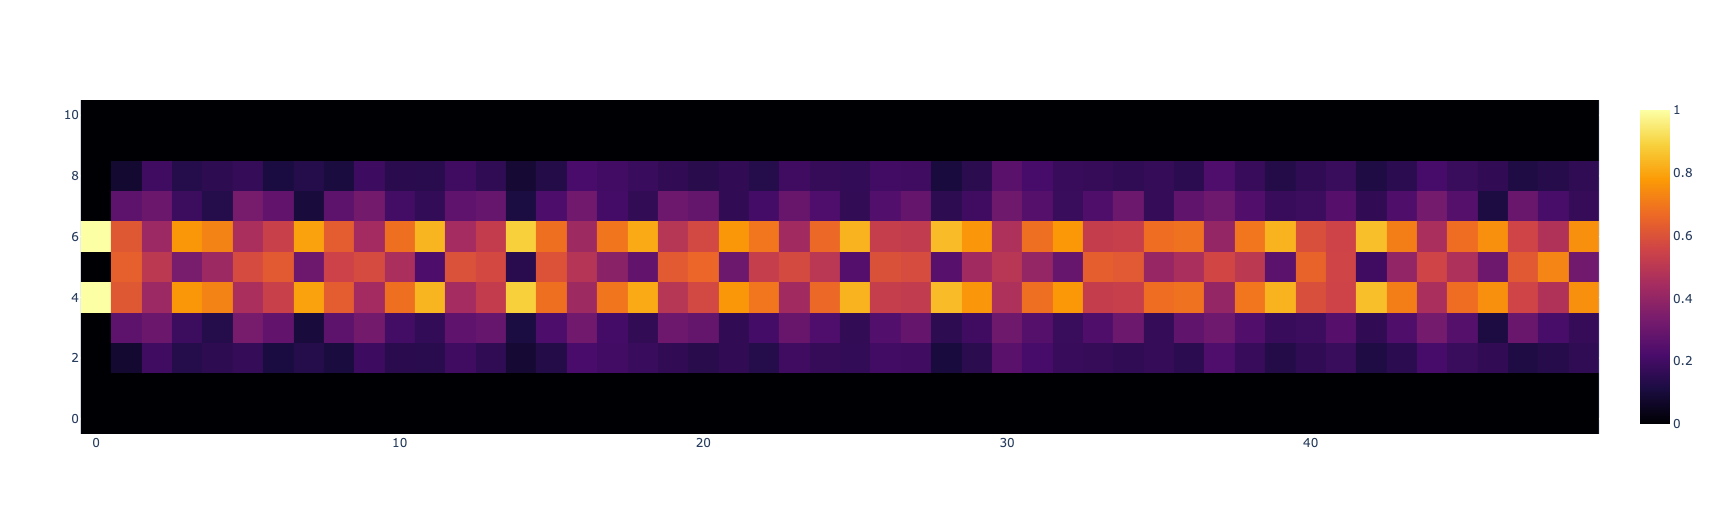
\includegraphics[width=\columnwidth]{graphics/blinker.png}
        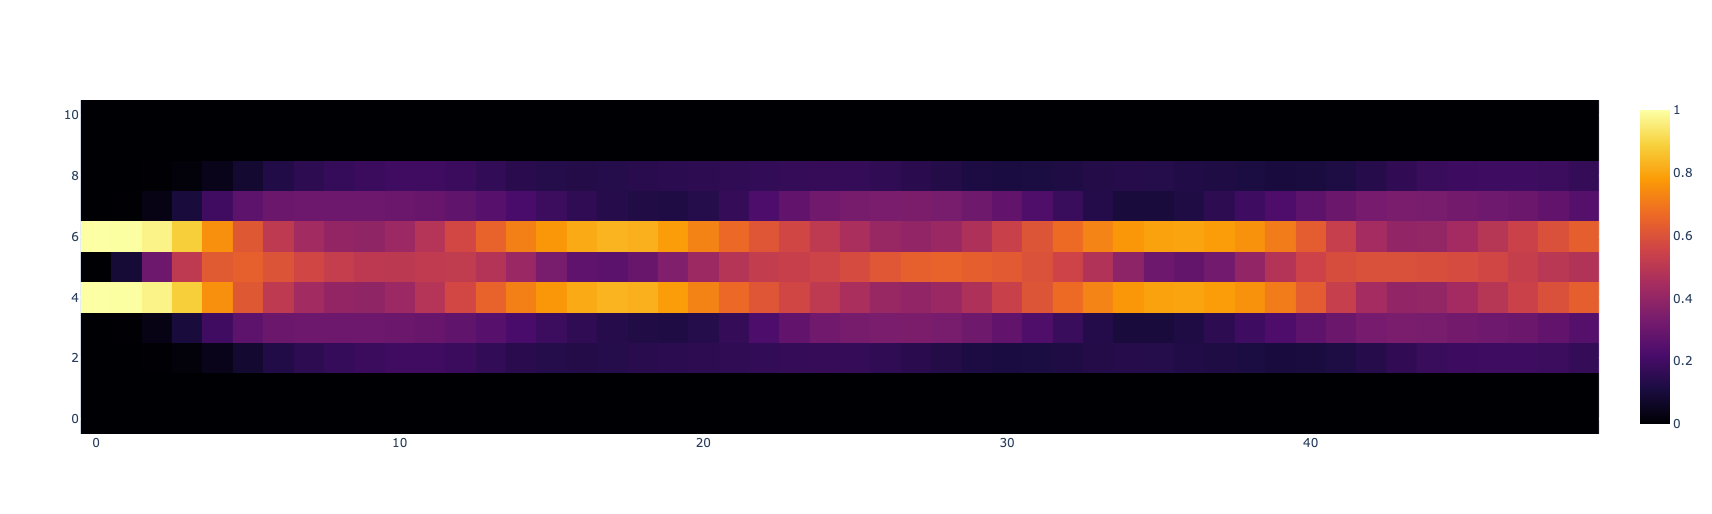
\includegraphics[width=\columnwidth]{graphics/blinker_slow.png}
    \column{.5\textwidth}
        \centering
        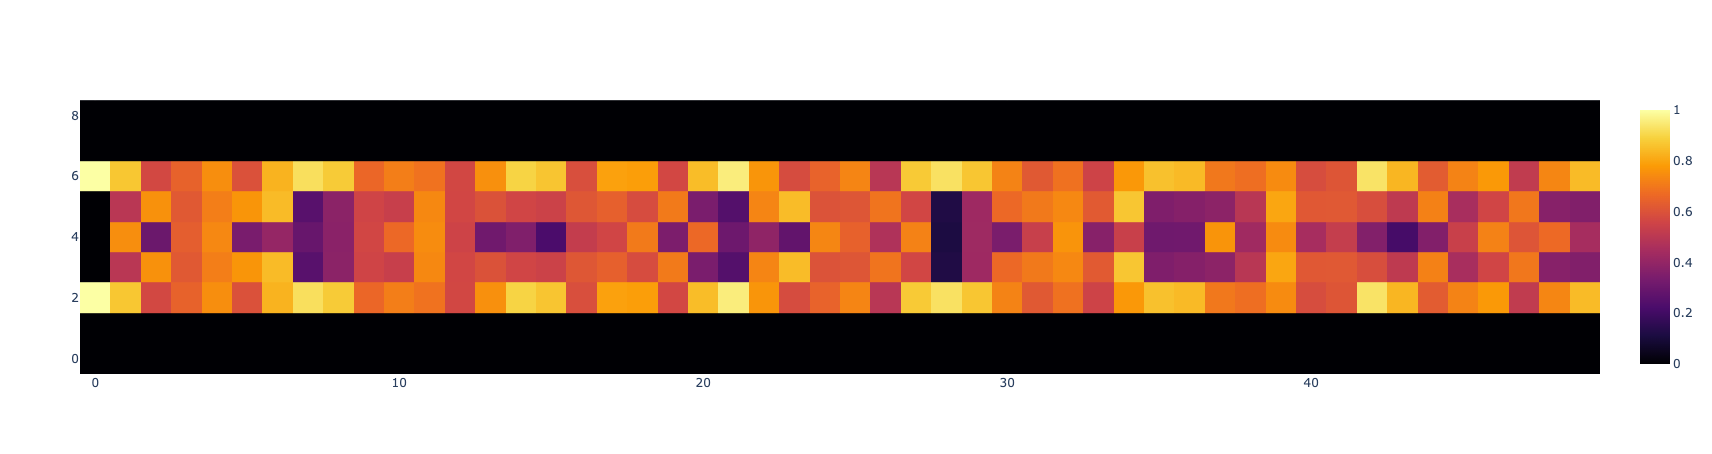
\includegraphics[width=\columnwidth]{graphics/wide_blinker.png}
        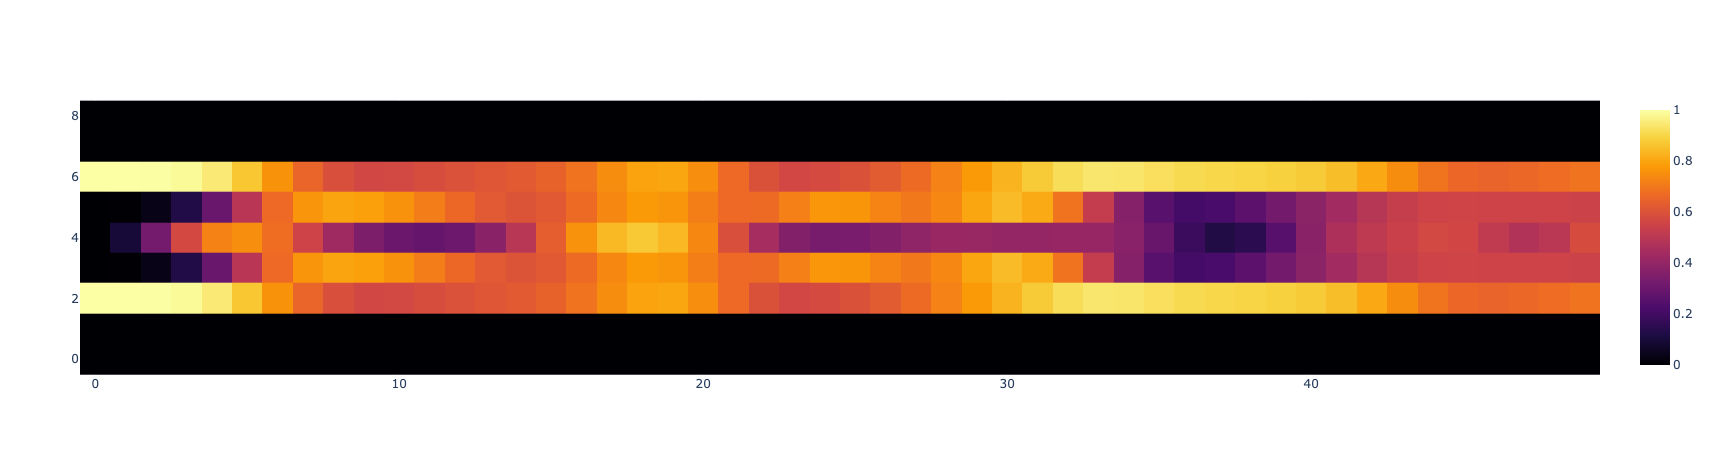
\includegraphics[width=\columnwidth]{graphics/wide_blinker_slow.png}
    \end{columns}
    \caption{Time evolution of the initial states $\ket{\psi}_0^{(left)}=\ket{0}^{\otimes4}\otimes\ket{101}\otimes\ket{0}^{\otimes4}$ and $\ket{\psi}_0^{(right)}=\ket{001000100}$ according to equation (\ref{eq:variableSingleTimeStepEvolution}) with $t^{(top)}=\frac{\pi}{2}$ and $t^{(bottom)}=\frac{\pi}{10}$ shown as the distribution of alive cells}
    \label{fig:variableSingleTimeStepEvolutionComparison}
    \end{figure}
    }
    \vspace{1000pt}
\end{frame}

\begin{frame}[t]{Entropy of entanglement}
    \onslide<2->{
    \begin{equation}
        \ket{\Psi_{AB}} = \ket{\psi_A}\ket{\psi_B}
        \label{eq:ketAB}
    \end{equation}
    \begin{equation}
        \rho_A = Tr_B(\ket{\Psi_{AB}}\bra{\Psi_{AB}})
        \label{eq:partialTrace}
    \end{equation}
    \begin{equation}
        \vonNeumannEntropy
        \label{eq:vonNeumannEntropy}
    \end{equation}
    }
    \onslide<3->{
    \begin{itemize}
        \item $S(\rho_A)$ is called the entropy of entanglement
        \item A measure of the degree of entanglement between subsystems $A$ and $B$
        \item $S(\rho_A) = 0 \Longrightarrow$ subsystems $A$ and $B$ are not entangled
    \end{itemize}
    }
    \onslide<4->{
    \begin{center}
        If $A$ represents one cell and $B$ represents the rest of the system, $S(\rho_A)$ is called the \textbf{single site entropy}.
    \end{center}
    }
\end{frame}

\begin{frame}{Single site entropy}
    \begin{equation}
        \vonNeumannEntropy
        \tag{\ref{eq:vonNeumannEntropy}}
    \end{equation}
    \onslide<2>{
    \begin{figure}
    \begin{columns}
    \column{.5\textwidth}
        \centering
        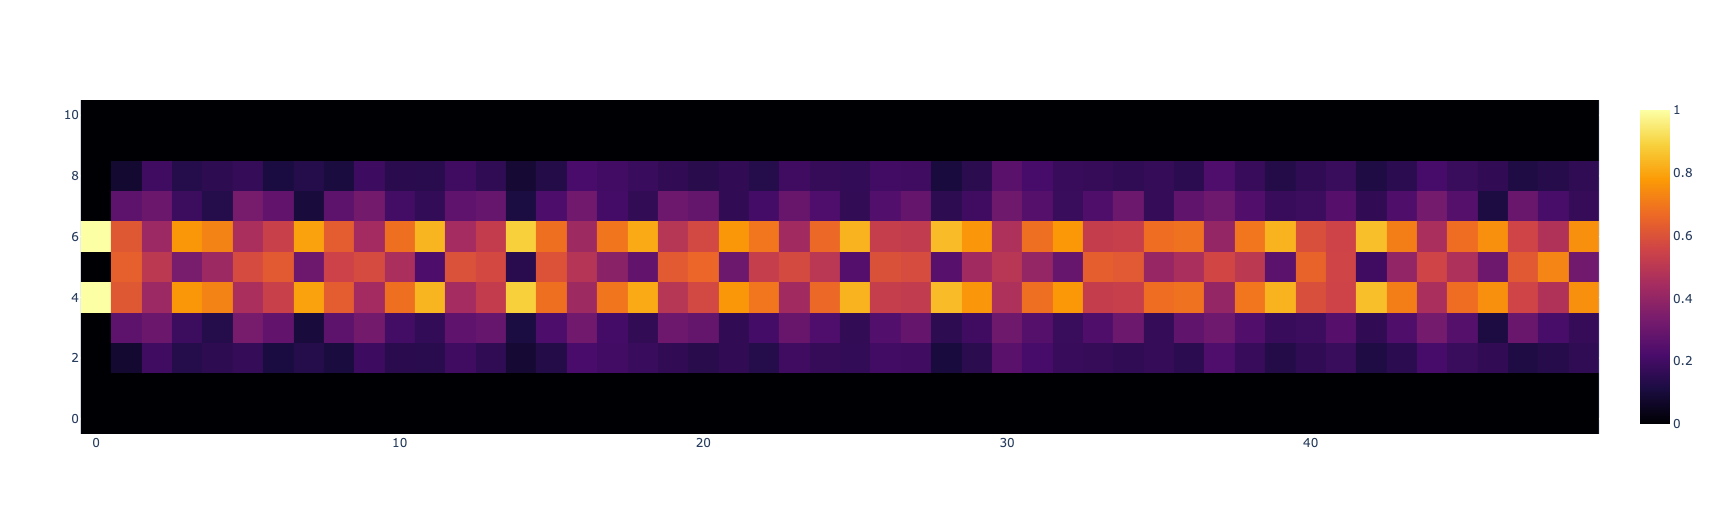
\includegraphics[width=\columnwidth]{graphics/blinker.png}
        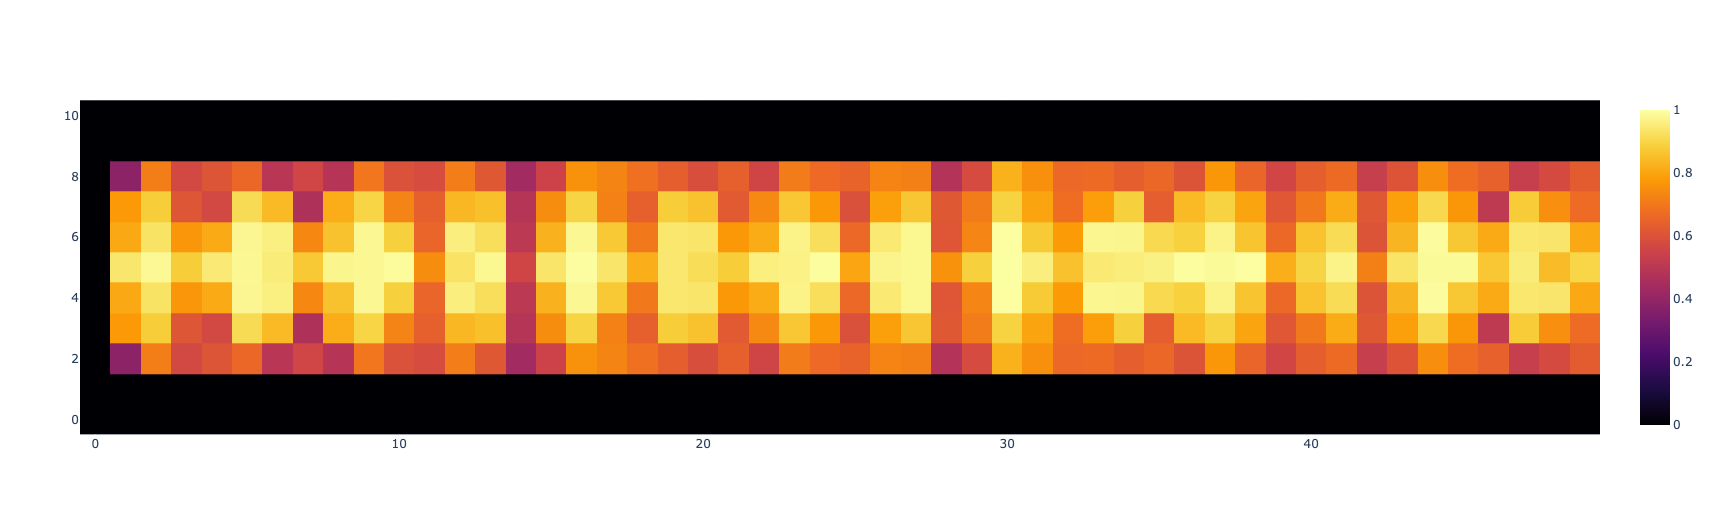
\includegraphics[width=\columnwidth]{graphics/blinker_sse.png}
    \column{.5\textwidth}
        \centering
        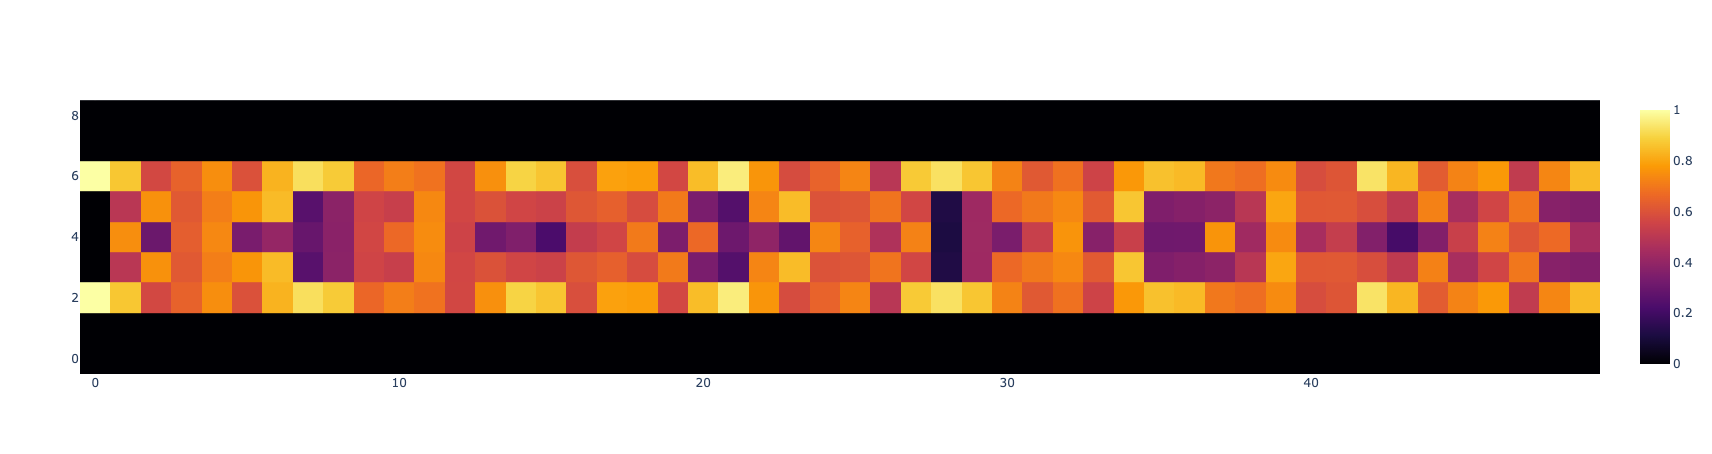
\includegraphics[width=\columnwidth]{graphics/wide_blinker.png}
        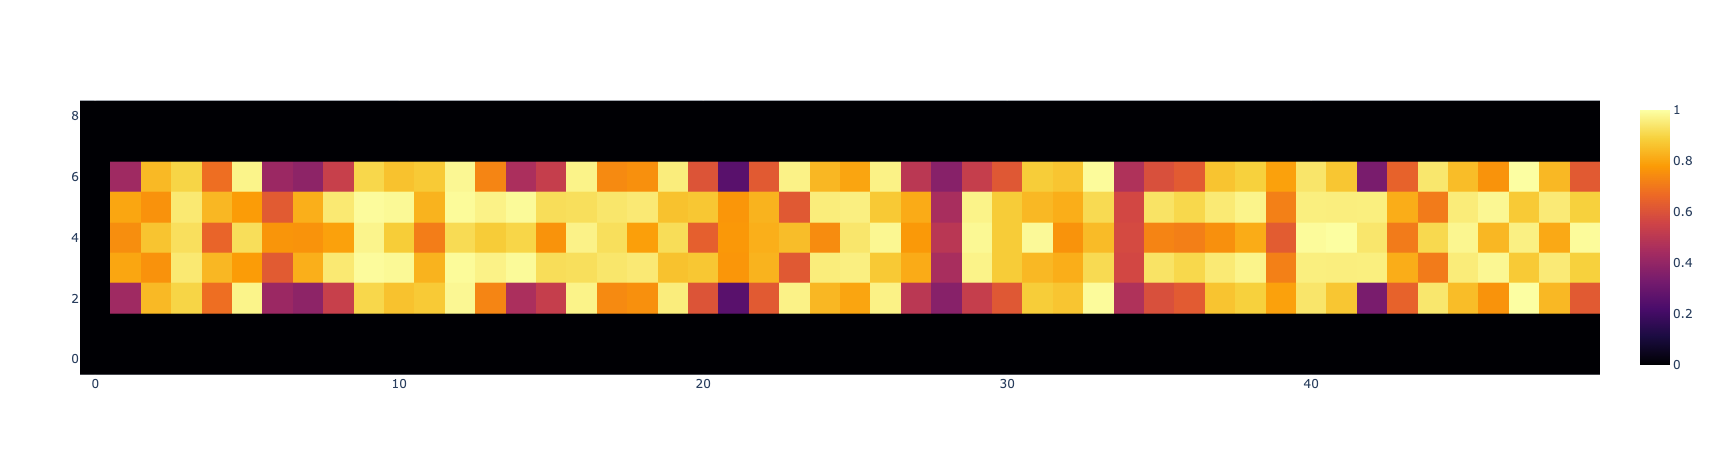
\includegraphics[width=\columnwidth]{graphics/wide_blinker_sse.png}
    \end{columns}
    \caption{Time evolution of the initial states $\ket{\psi}_0^{(left)}=\ket{0}^{\otimes4}\otimes\ket{101}\otimes\ket{0}^{\otimes4}$ and $\ket{\psi}_0^{(right)}=\ket{001000100}$ shown as the distribution of alive cells (top) and single site entropy (bottom)}
    \label{fig:variableSingleTimeStepEvolutionComparison}
    \end{figure}
    }
    \vspace{1000pt}
\end{frame}

\begin{frame}{Wolfram Code}
    \begin{center}
        A naming system to define the rules of a cellular automaton
    \end{center}
    \vspace{10pt}
    \onslide<2->{
    \begin{center}
        Rule $150$:\\"A cell is flipped if the number of alive cells among its nearest neighbors is $1$"
    \end{center}
    }
    \vspace{2pt}
    \onslide<3->{
    \begin{center}
        \begin{tabular}{ c c c c c c c c }
         1 {\color{red}1} 1 & 1 {\color{TUM-blue}1} 0 & 1 {\color{red}0} 1 & 1 {\color{TUM-blue}0} 0 & 0 {\color{TUM-blue}1} 1 & 0 {\color{red}1} 0 & 0 {\color{TUM-blue}0} 1 & 0 {\color{red}0} 0 \\
         {\color{red}1} & {\color{TUM-blue}0} & {\color{red}0} & {\color{TUM-blue}1} & {\color{TUM-blue}0} & {\color{red}1} & {\color{TUM-blue}1} & {\color{red}0}
        \end{tabular}
    \end{center}
    }
    \vspace{2pt}
    \onslide<4->{
    \begin{center}
        The corresponding wolfram code for this rule is $10010110b=\textbf{150}$
    \end{center}
    }
    \onslide<5->{
    \begin{center}
        The wolfram code for rule-$F_{12}$ is $2266898040$
    \end{center}
    }
\end{frame}

\begin{frame}[t]{Changing the rules}
    \begin{equation}
        \hamiltonianPaper
        \tag{\ref{eq:hamiltonianPaper}}
    \end{equation}
    \onslide<2->{
    \vspace{10pt}
    \begin{center}
        From this specific Hamiltonian, other Hamiltonians corresponding to different rules can be derived. A more general form looks like
    \end{center}
    \vspace{10pt}
    \begin{equation}
        \hamiltonianGeneral
        \label{eq:hamiltonianGeneral}
    \end{equation}
    }
    \only<3->{
    \begin{itemize}
        \onslide<3->{
        \item $\hat{N}_i$ defines how many neighbors are considered and how many of them need to be alive to flip a cell
        }
        \onslide<4->{
        \item The bounds of the summation index $i$ depend on $\hat{N}_i$ and on the the boundary conditions used
        }
    \end{itemize}
    }
    \vspace{1000pt}
\end{frame}

\begin{frame}[t]{Rule 150}
    \begin{equation}
        \hamiltonianGeneral
        \tag{\ref{eq:hamiltonianGeneral}}
    \end{equation}
    \only<2>{
    \begin{figure}
    \begin{columns}
    \column{.5\textwidth}
        \centering
        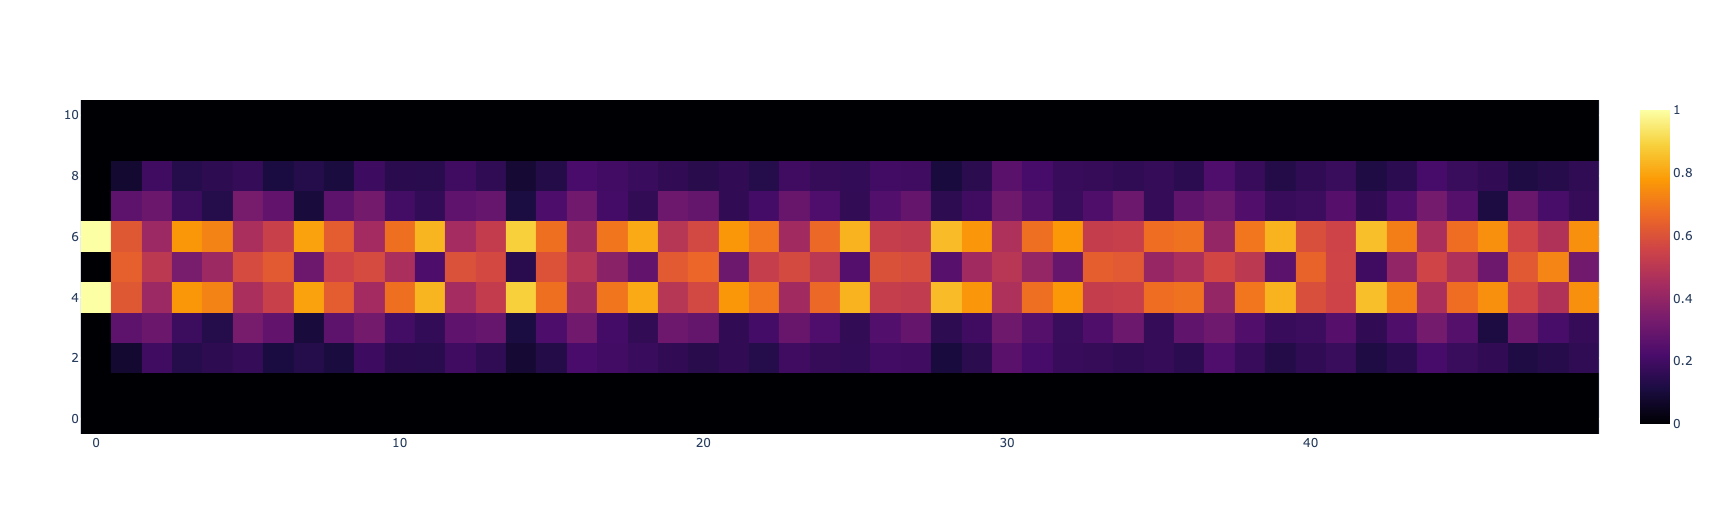
\includegraphics[width=\columnwidth]{graphics/blinker.png}
        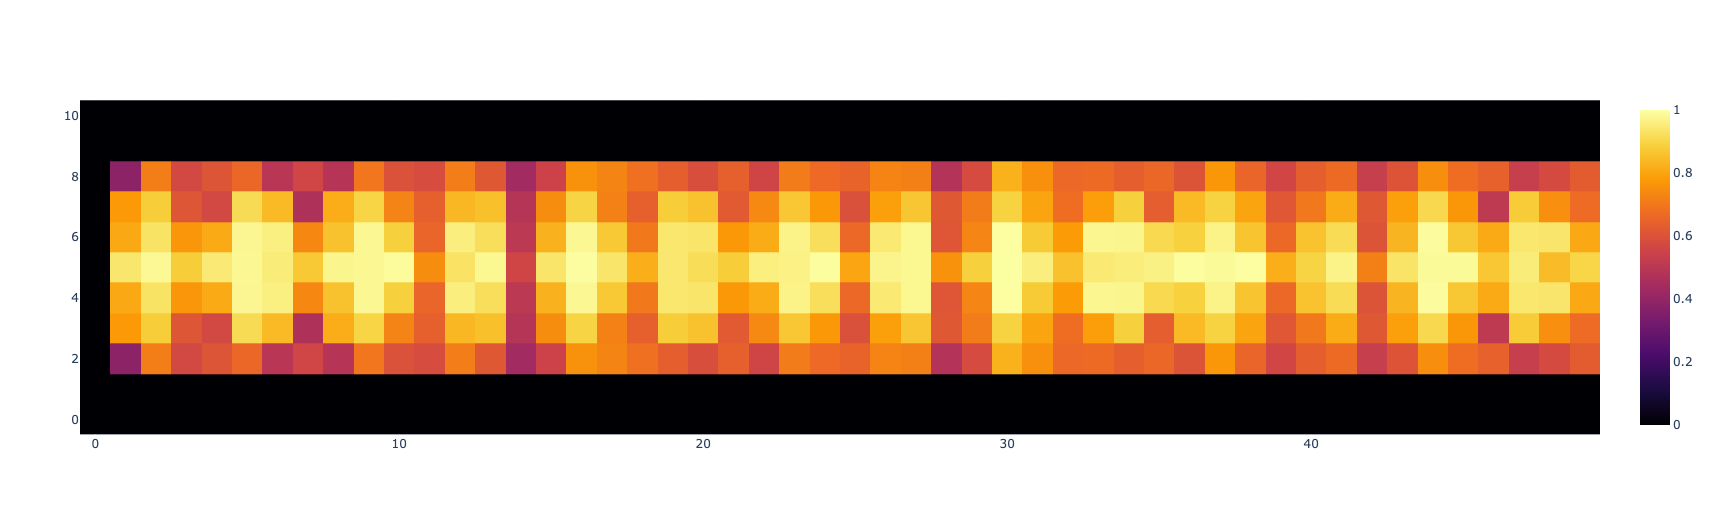
\includegraphics[width=\columnwidth]{graphics/blinker_sse.png}
    \column{.5\textwidth}
        \centering
        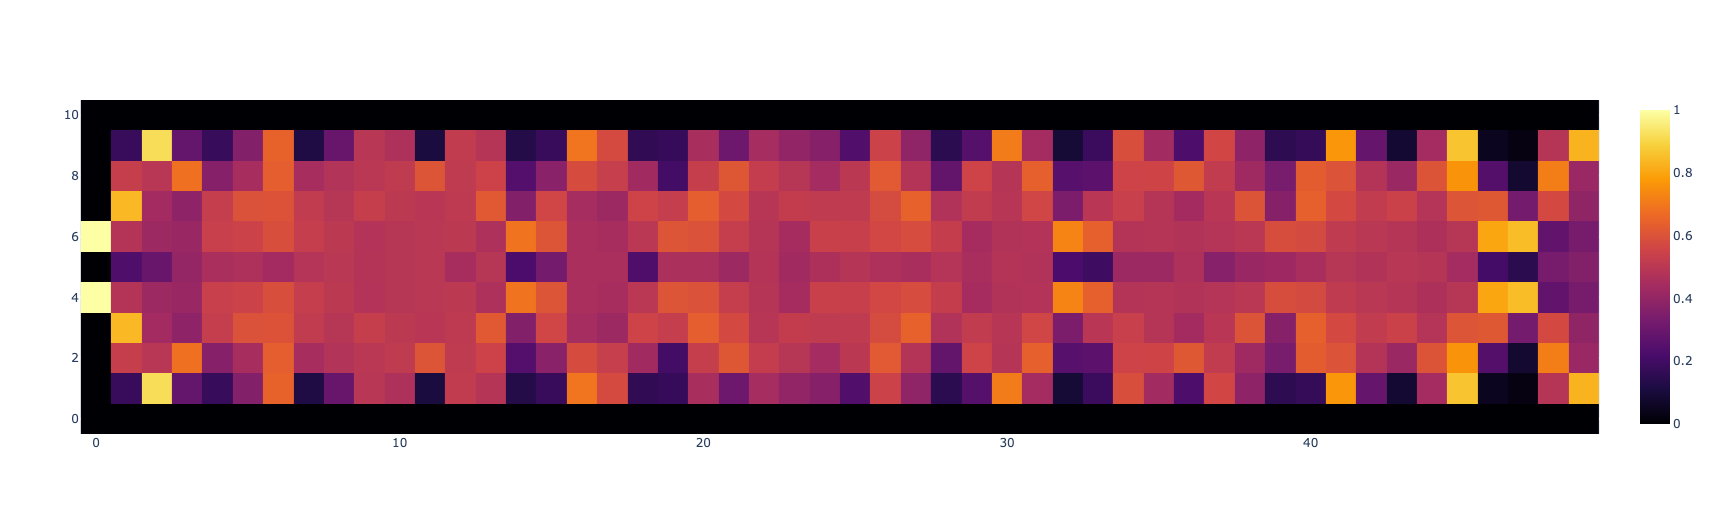
\includegraphics[width=\columnwidth]{graphics/blinker_150.png}
        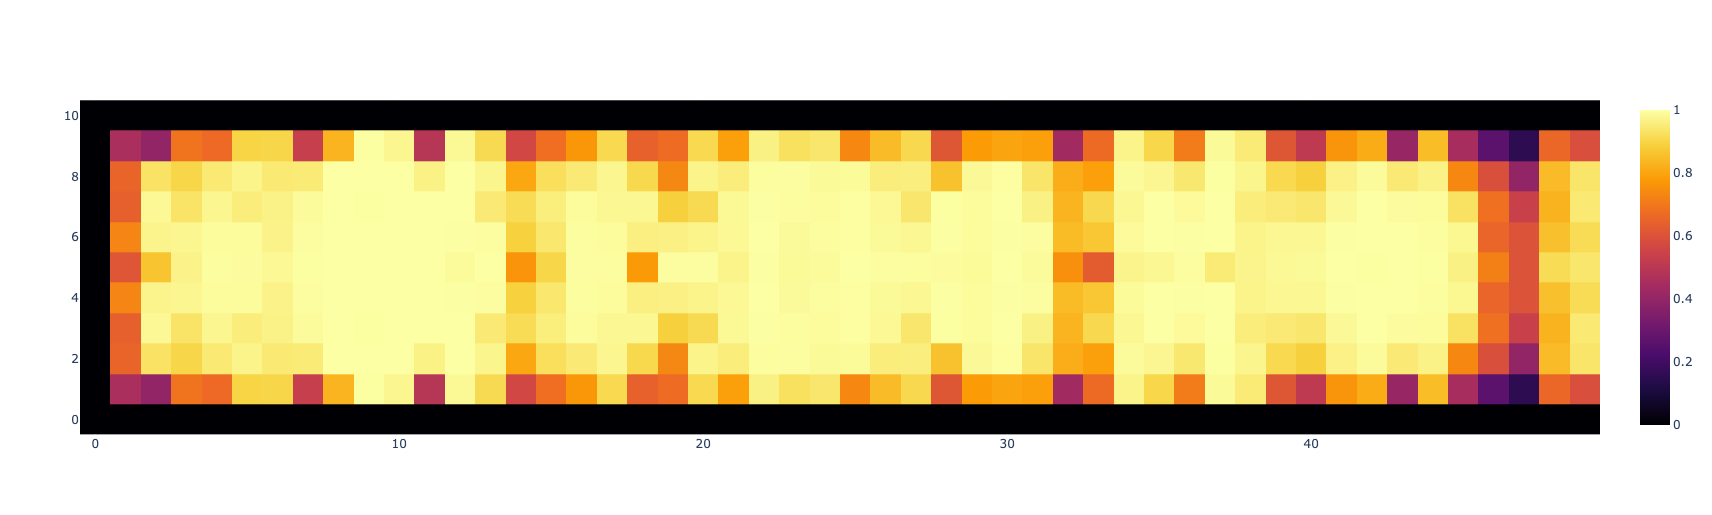
\includegraphics[width=\columnwidth]{graphics/blinker_150_sse.png}
    \end{columns}
    \caption{Time evolution of the initial state $\ket{\psi}_0=\ket{0}^{\otimes4}\otimes\ket{101}\otimes\ket{0}^{\otimes4}$ according to rule $F_{12}$ (left) and rule $150$ (right) shown as the distribution of alive cells (top) and single site entropy (bottom)}
    \end{figure}
    }
    \only<3>{
    \begin{figure}
    \begin{columns}
    \column{.5\textwidth}
        \centering
        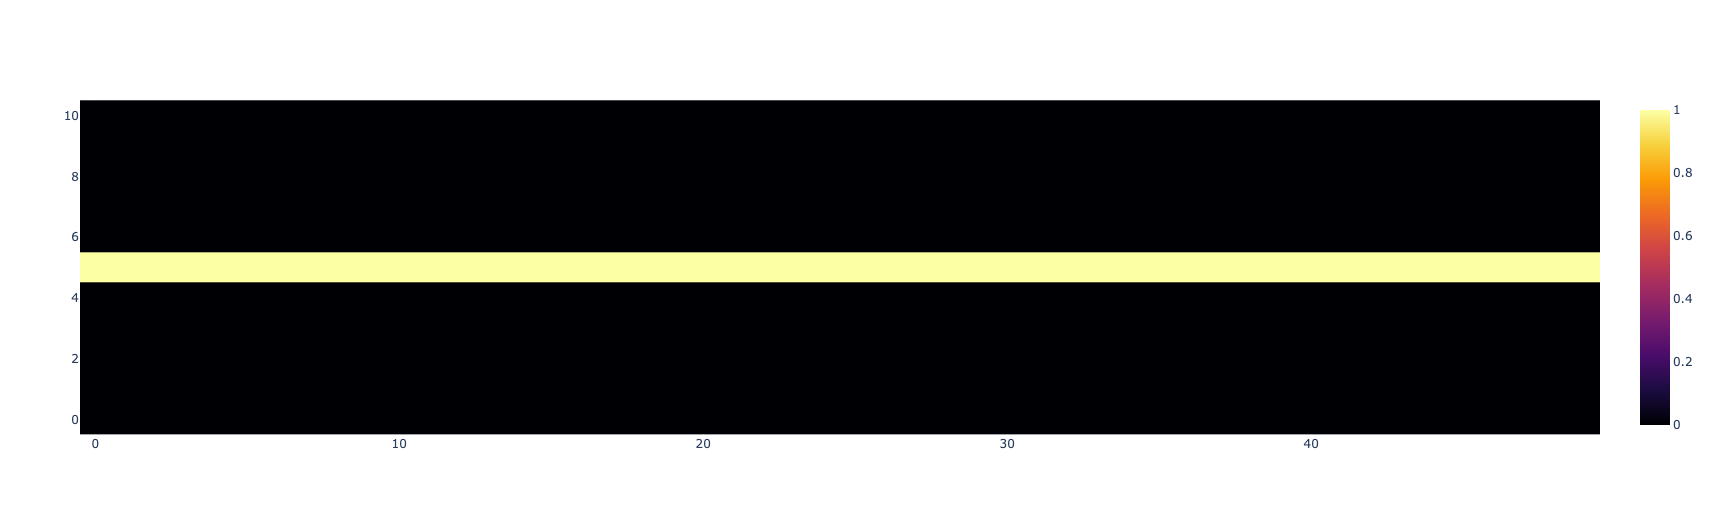
\includegraphics[width=\columnwidth]{graphics/single_f12.png}
        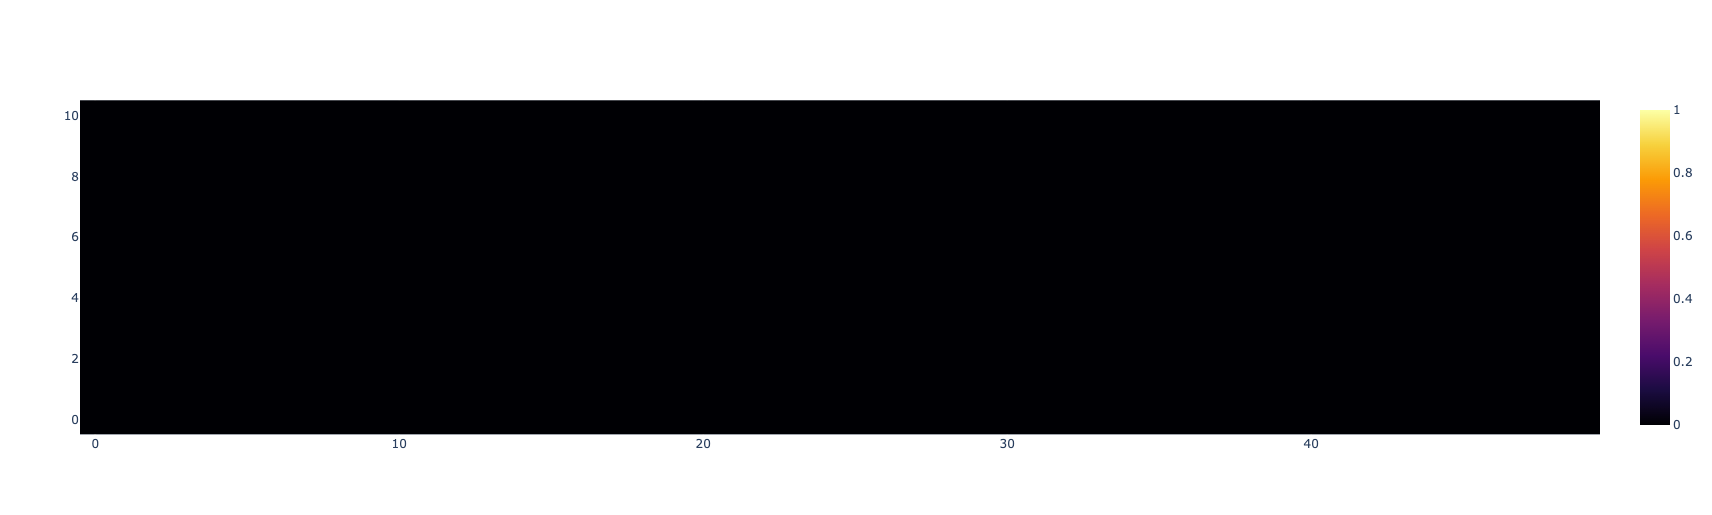
\includegraphics[width=\columnwidth]{graphics/single_f12_sse.png}
    \column{.5\textwidth}
        \centering
        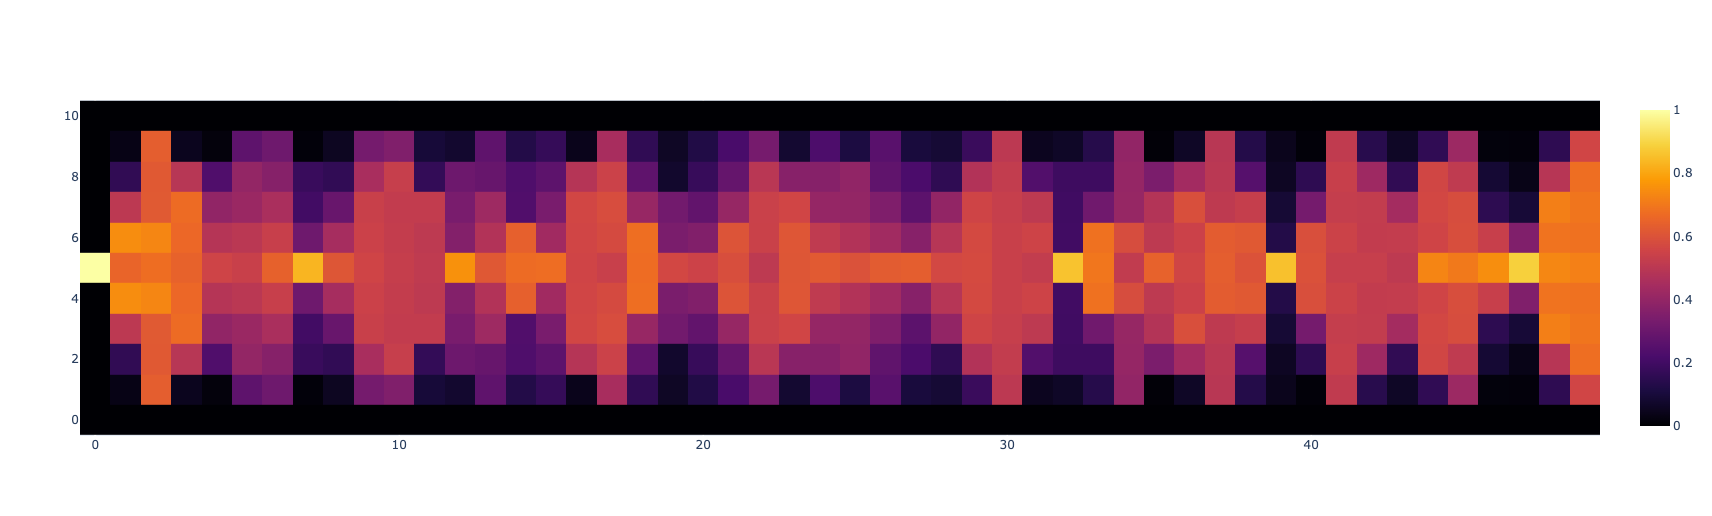
\includegraphics[width=\columnwidth]{graphics/single_150.png}
        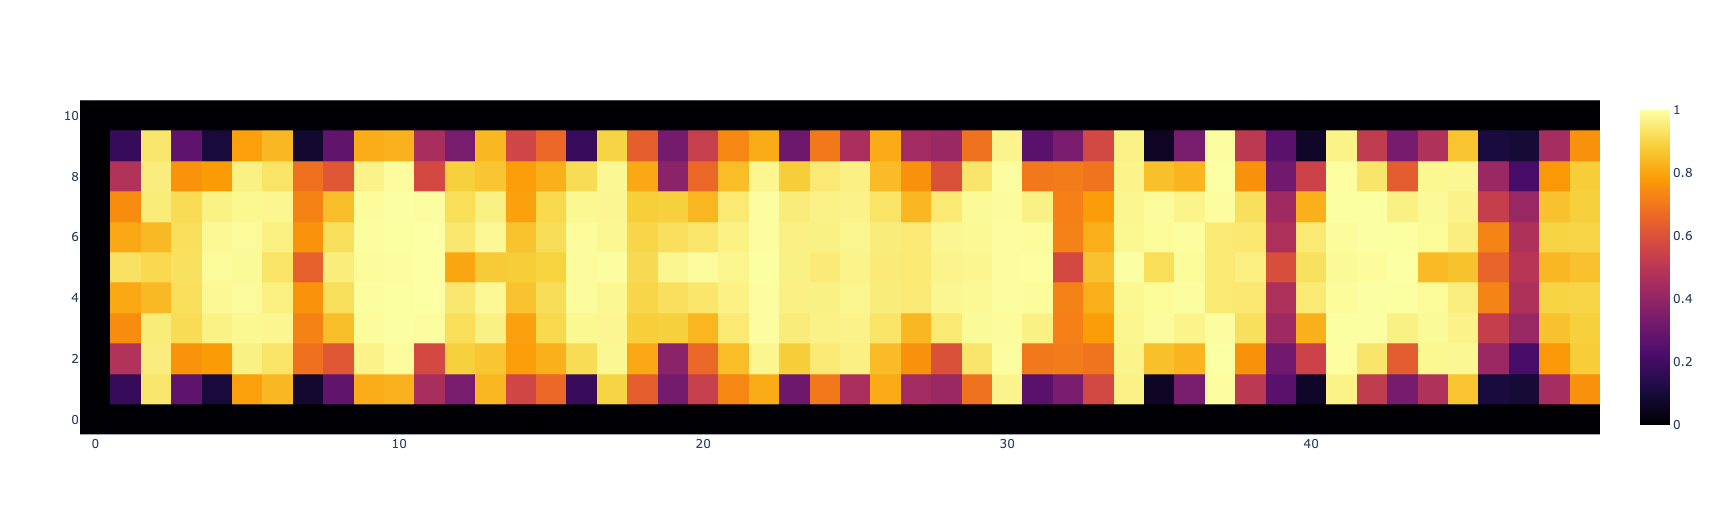
\includegraphics[width=\columnwidth]{graphics/single_150_sse.png}
    \end{columns}
    \caption{Time evolution of the initial state $\ket{\psi}_0=\ket{0}^{\otimes5}\otimes\ket{1}\otimes\ket{0}^{\otimes5}$ according to rule $F_{12}$ (left) and rule $150$ (right) shown as the distribution of alive cells (top) and single site entropy (bottom)}
    \end{figure}
    }
    \only<4>{
    \begin{figure}
    \centering
    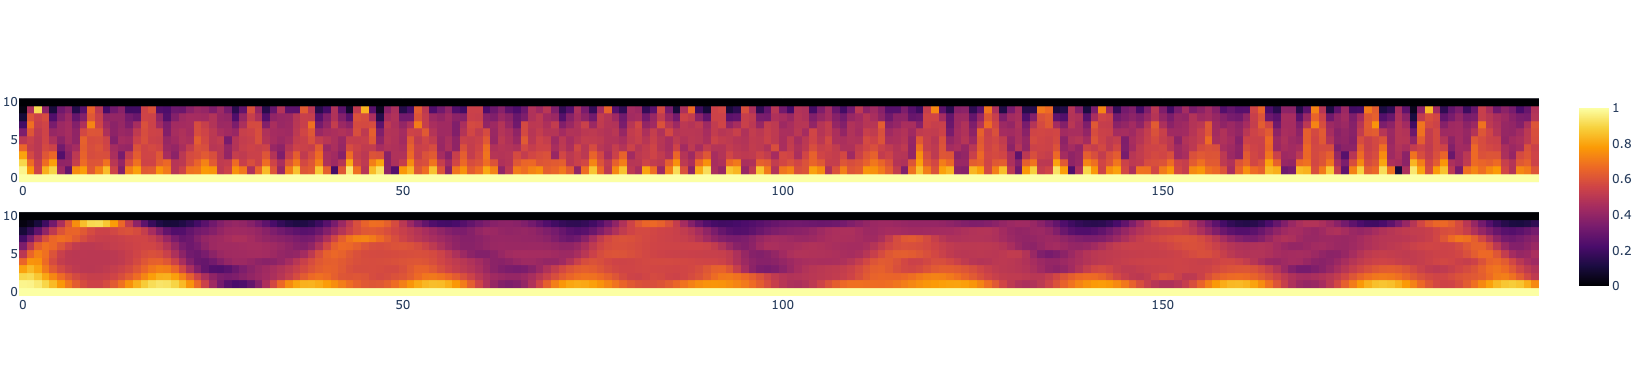
\includegraphics[width=\textwidth]{graphics/gradient_150_both.png}
    \caption{Time evolution of the initial state $\ket{\psi}_0=\bigotimes_{k = 0}^{N - 1}\left[R_x\left(\pi\frac{k}{N - 1}\right)\ket{1}\right]$, with $R_x(\theta)$ the x-rotation gate and $N=11$, according to rule $150$ with $t^{(top)}=\frac{\pi}{2}$ and $t^{(bottom)}=\frac{\pi}{10}$ shown as the distribution of alive cells}
    \end{figure}
    }
    \vspace{1000pt}
\end{frame}

\begin{frame}[t]{The Quantum Game of Life}
    \onslide<2->{
    \begin{columns}
    \column{.2\textwidth}
    \vspace{10pt}
    \begin{center}
        Classical
    \end{center}
    \vspace{10pt}
    \begin{center}
        Quantum
    \end{center}
    \vspace{10pt}
    \begin{center}
        Rounded
    \end{center}
    \vspace{5pt}
    \begin{center}
        single site entropy
    \end{center}
    \column{.8\textwidth}
    % \only<1>{
    % \begin{itemize}
    %     \item Row 1: Distribution of alive cells in the classical game of life
    %     \item Row 2: Distribution of alive cells in the quantum game of life
    %     \item Row 3: Rounded distribution of alive cells in the quantum game of life
    %     \item Row 4: Single site entropy
    % \end{itemize}
    % }
    \only<2>{
    \begin{figure}
        \centering
        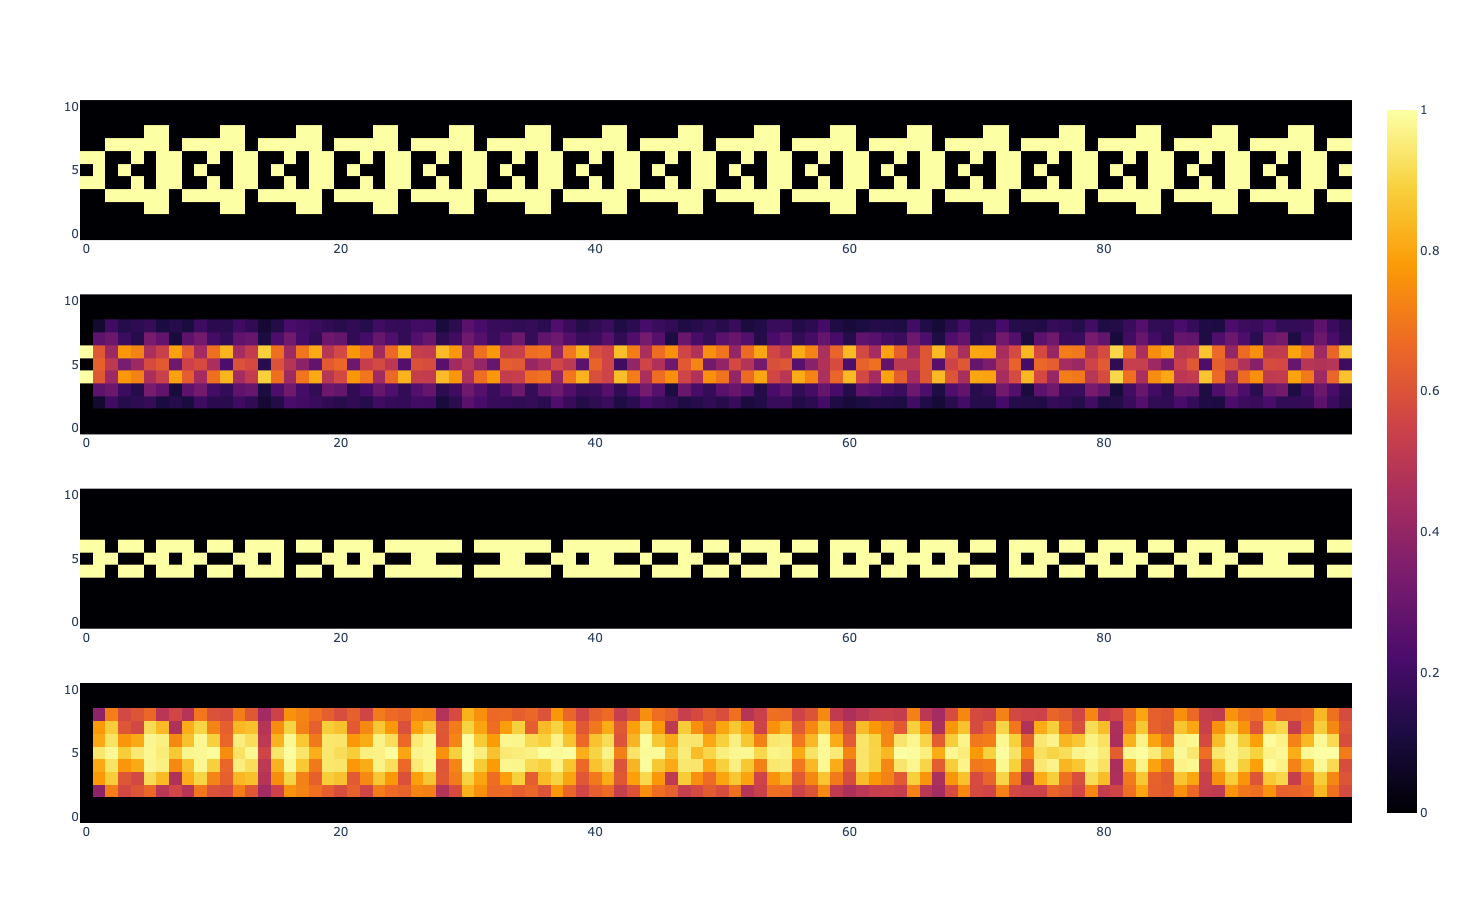
\includegraphics[width=\columnwidth]{graphics/blinker_f12_all.png}
    \end{figure}
    }
    \only<3>{
    \begin{figure}
        \centering
        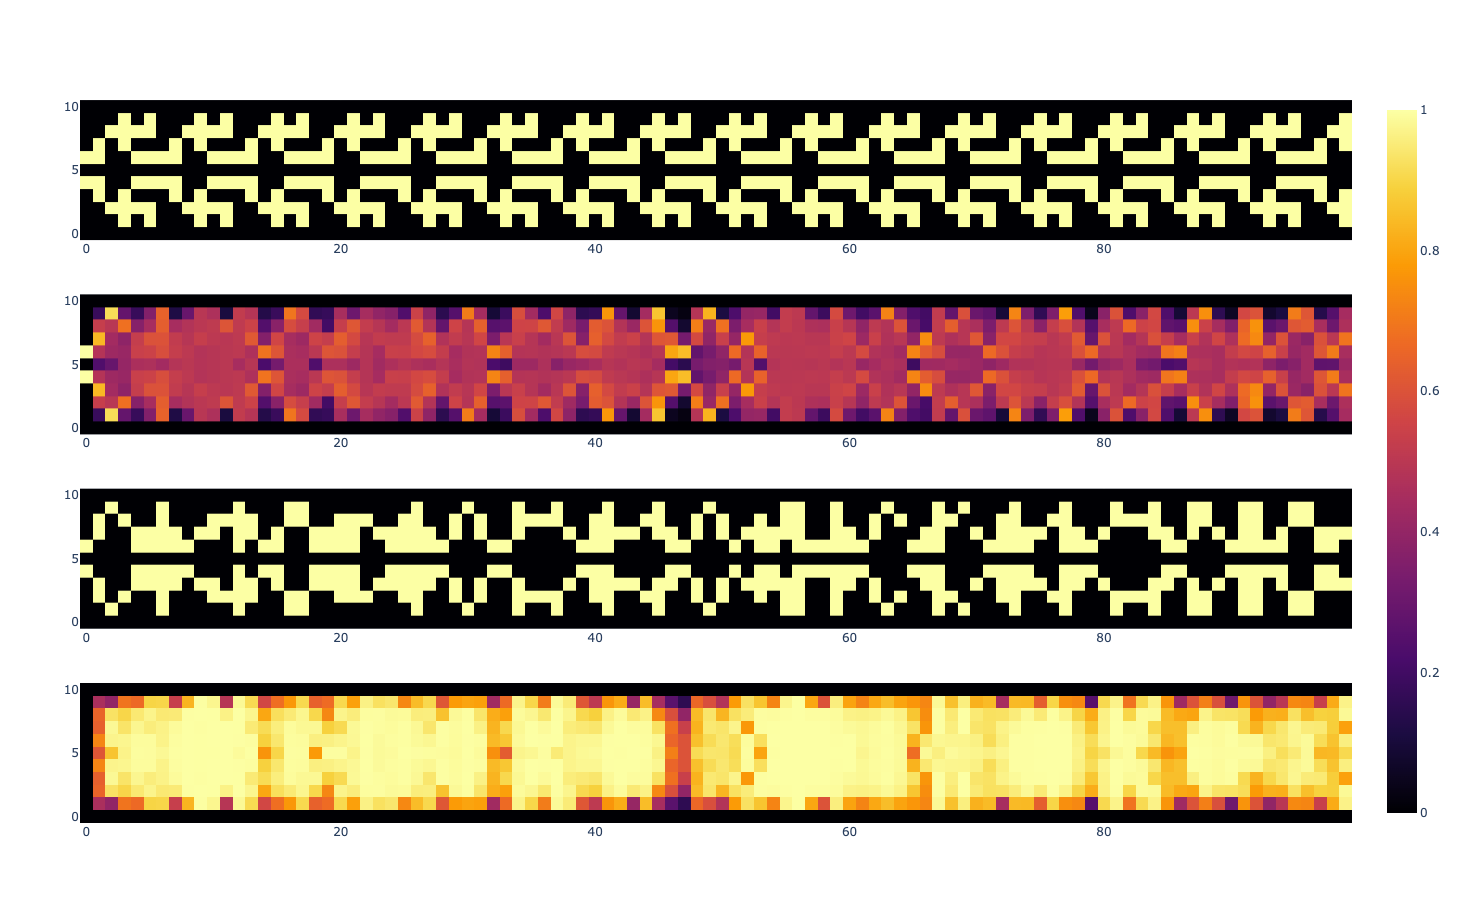
\includegraphics[width=\columnwidth]{graphics/blinker_150_all.png}
    \end{figure}
    }
    \only<4>{
    \begin{figure}
        \centering
        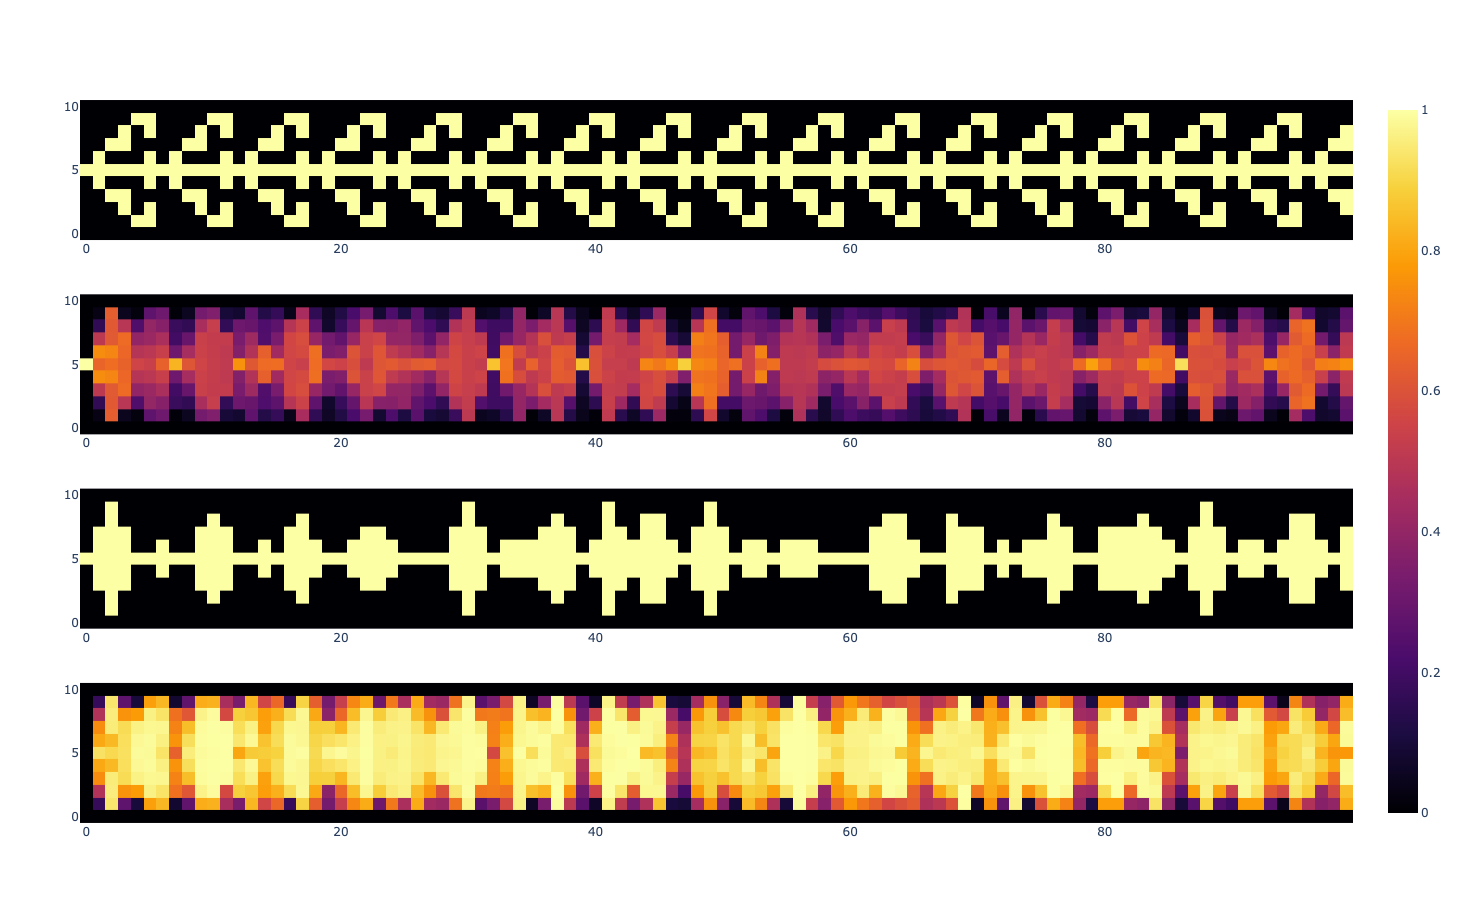
\includegraphics[width=\columnwidth]{graphics/single_150_all.png}
    \end{figure}
    }
    \only<5>{
    \begin{figure}
        \centering
        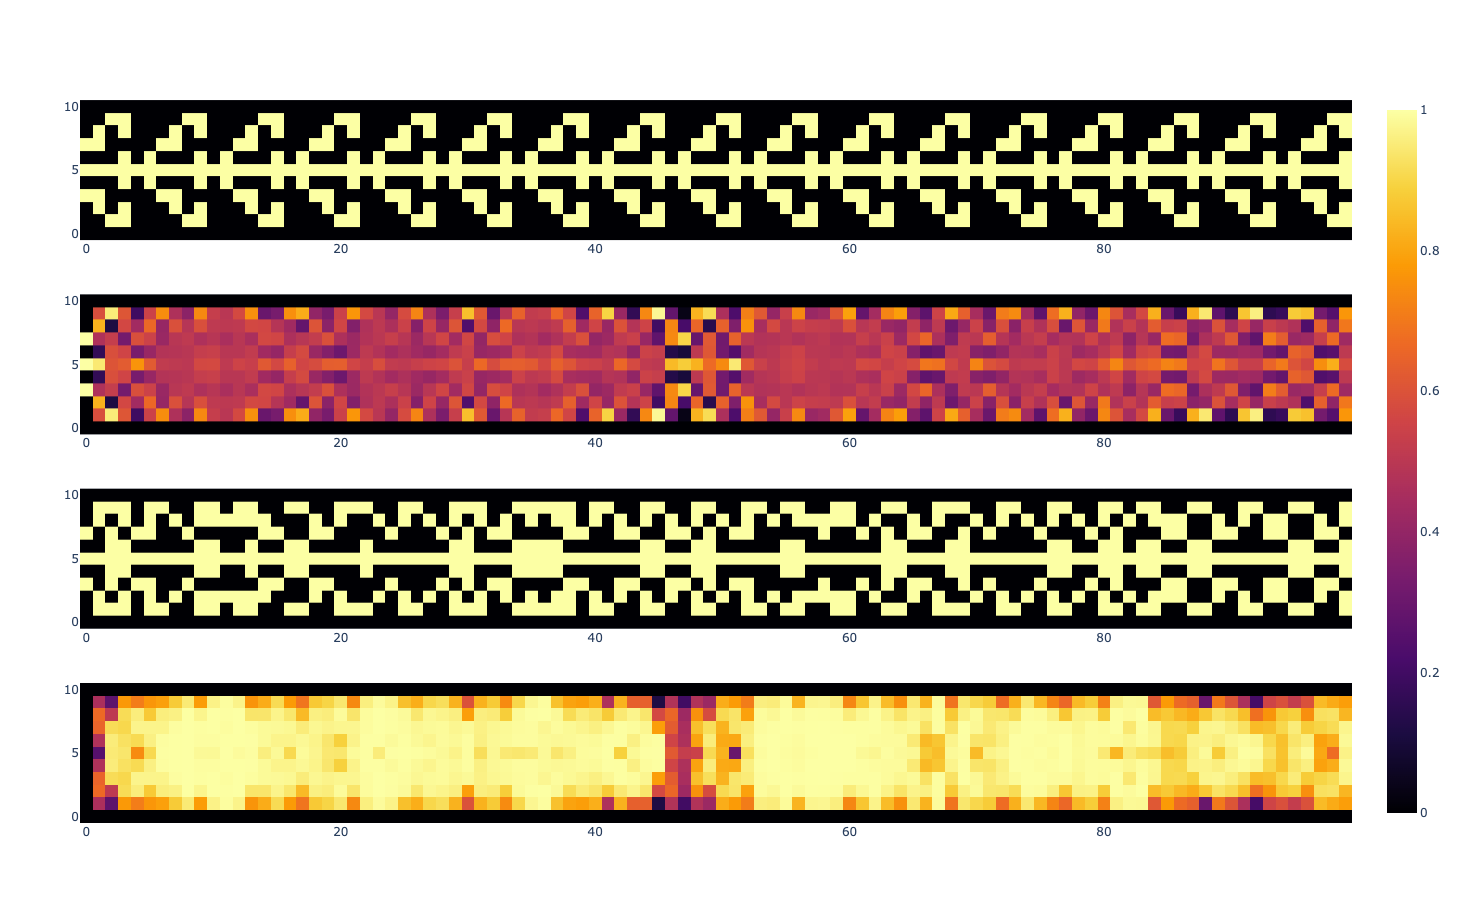
\includegraphics[width=\columnwidth]{graphics/triple_150_all.png}
    \end{figure}
    }
    \only<6>{
    \begin{figure}
        \centering
        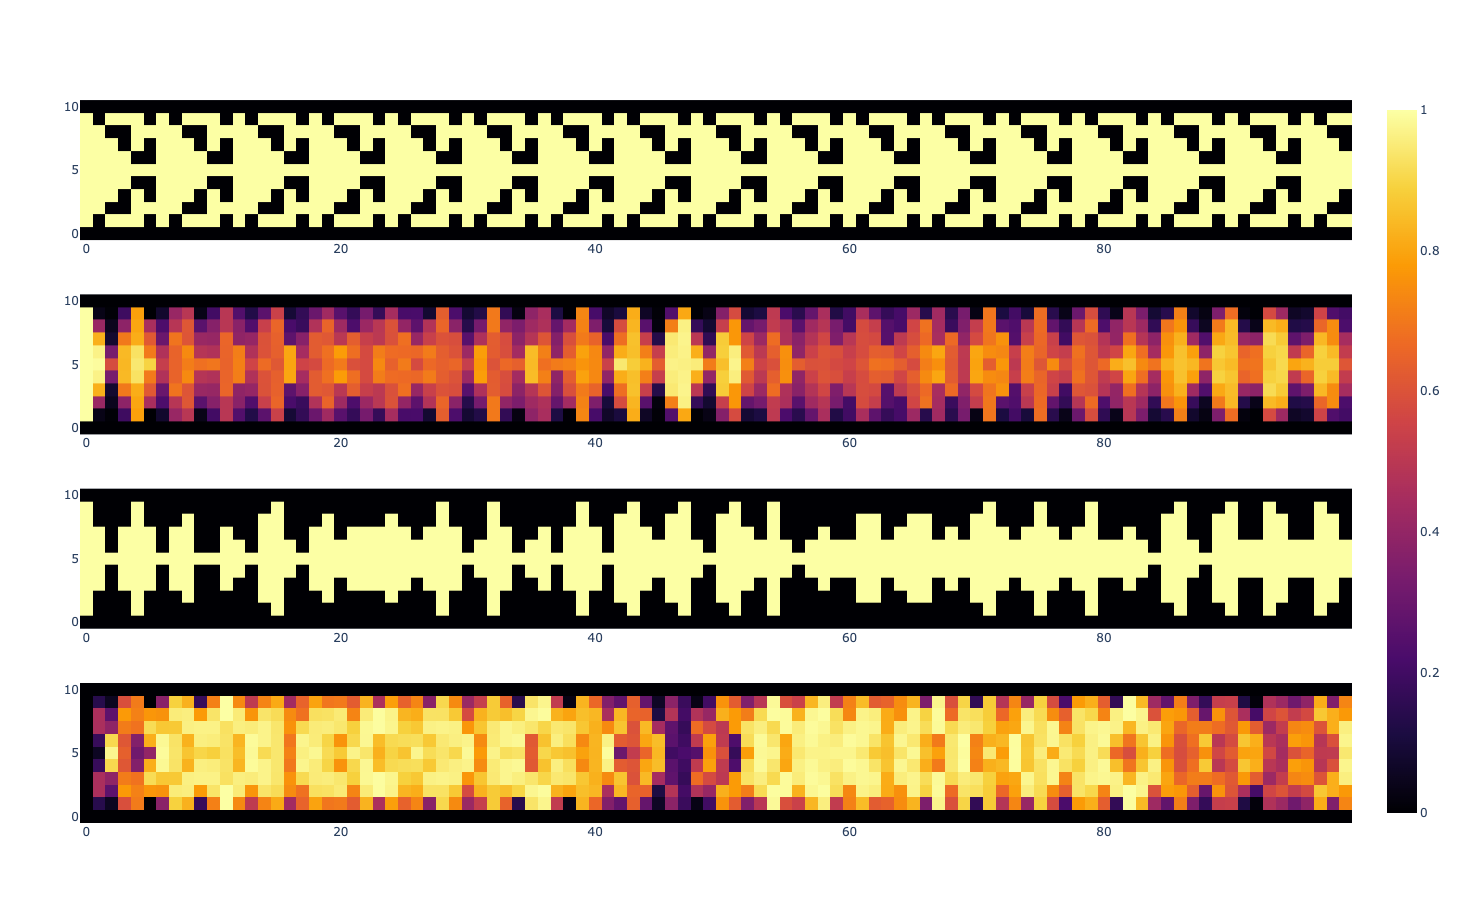
\includegraphics[width=\columnwidth]{graphics/all_ket_1_but_outer_all.png}
    \end{figure}
    }
    \only<7>{
    \begin{figure}
        \centering
        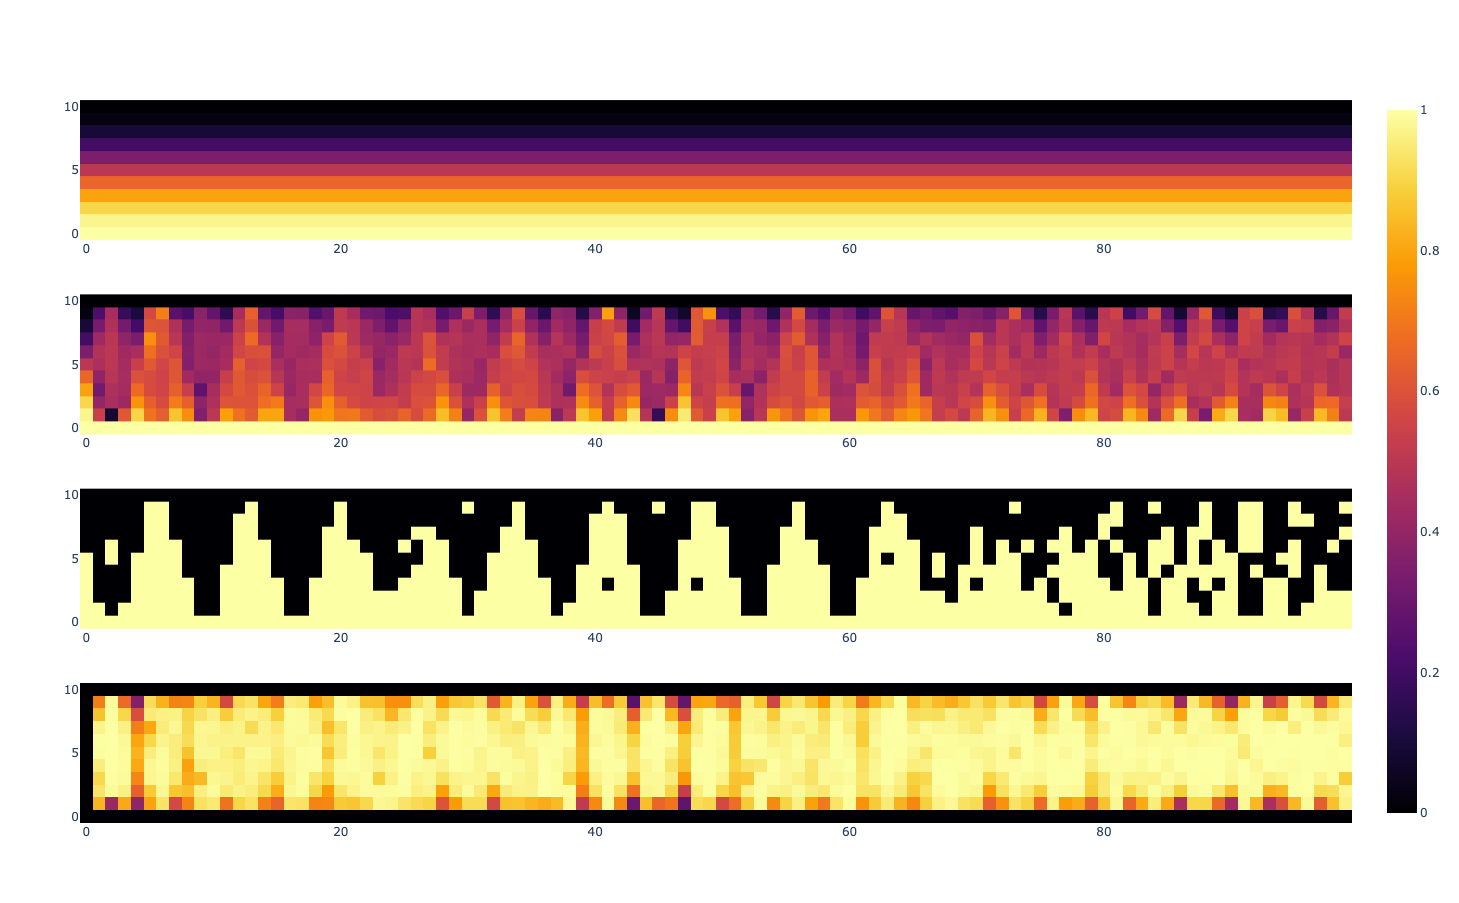
\includegraphics[width=\columnwidth]{graphics/gradient_150_all.png}
    \end{figure}
    }
    \only<8>{
    \begin{figure}
        \centering
        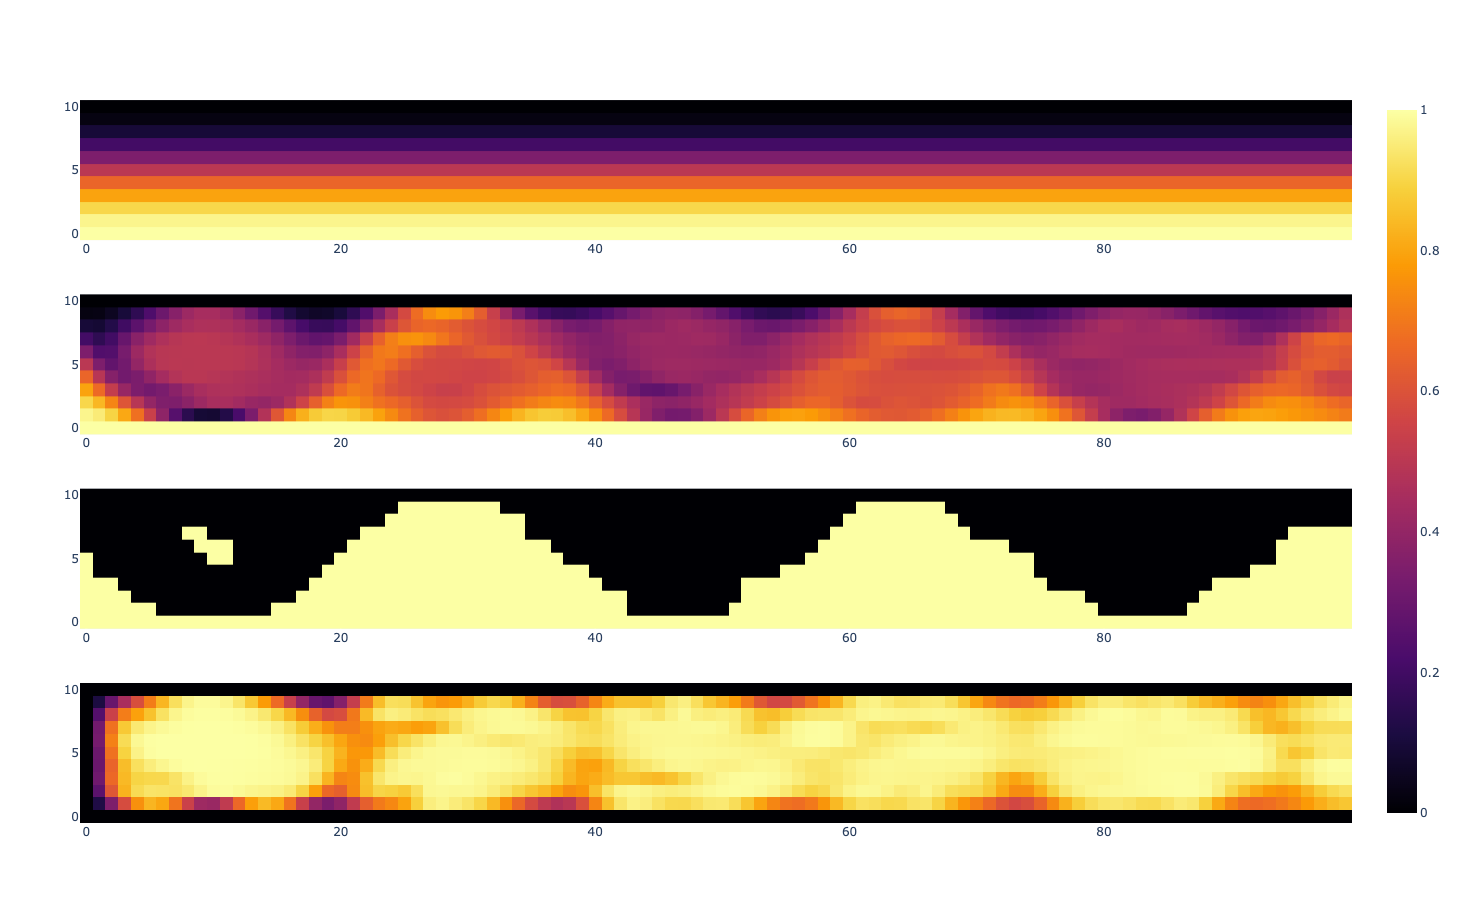
\includegraphics[width=\columnwidth]{graphics/gradient_150_slow_all.png}
    \end{figure}
    }
    \only<9>{
    \begin{figure}
        \centering
        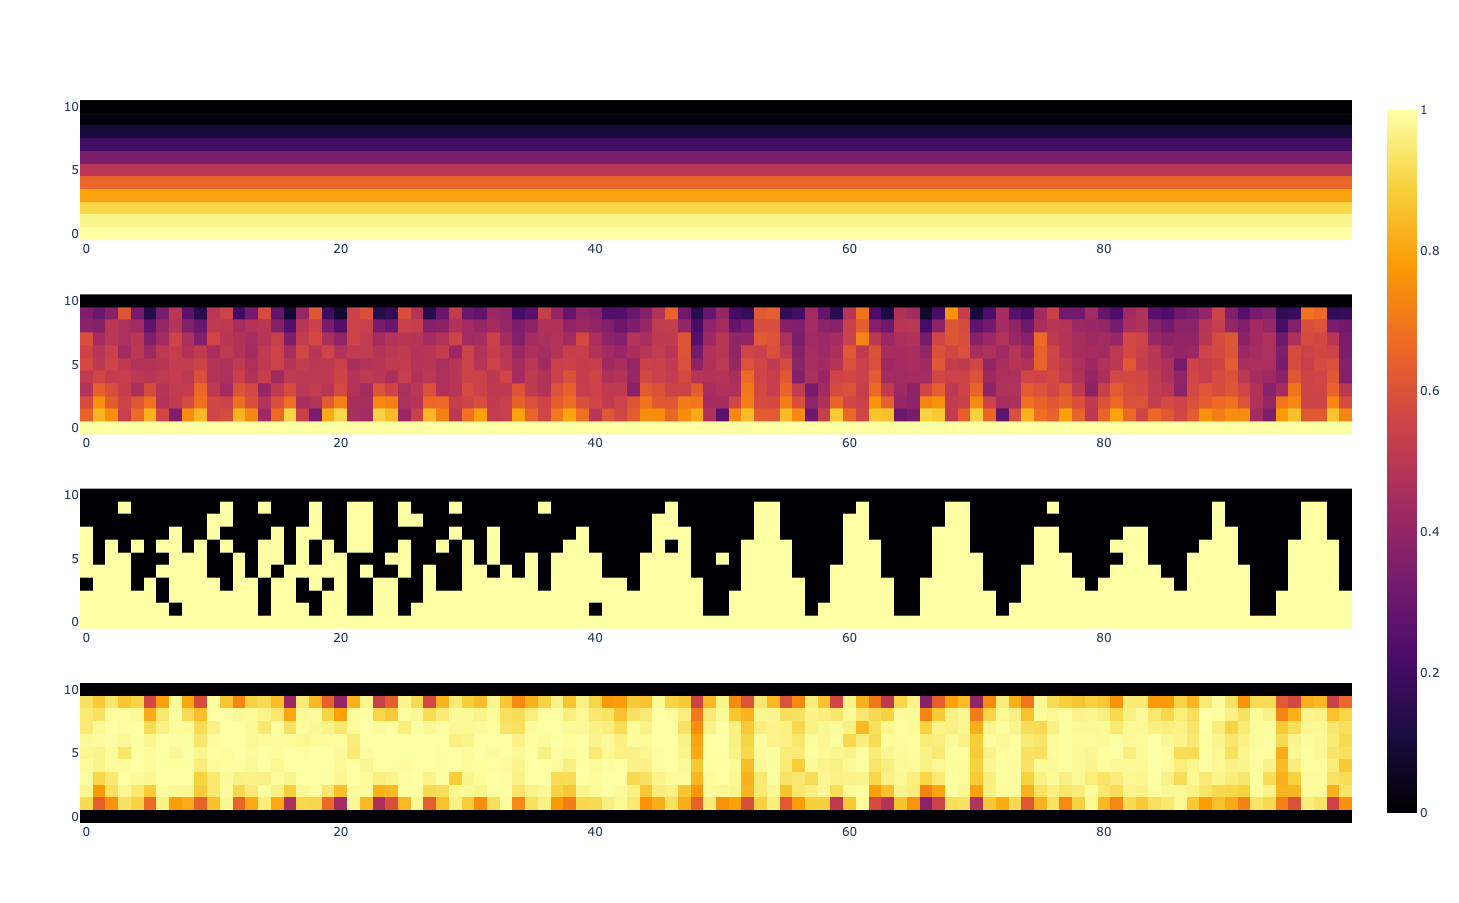
\includegraphics[width=\columnwidth]{graphics/gradient_150_from70_all.png}
    \end{figure}
    }
    \only<10>{
    \begin{figure}
        \centering
        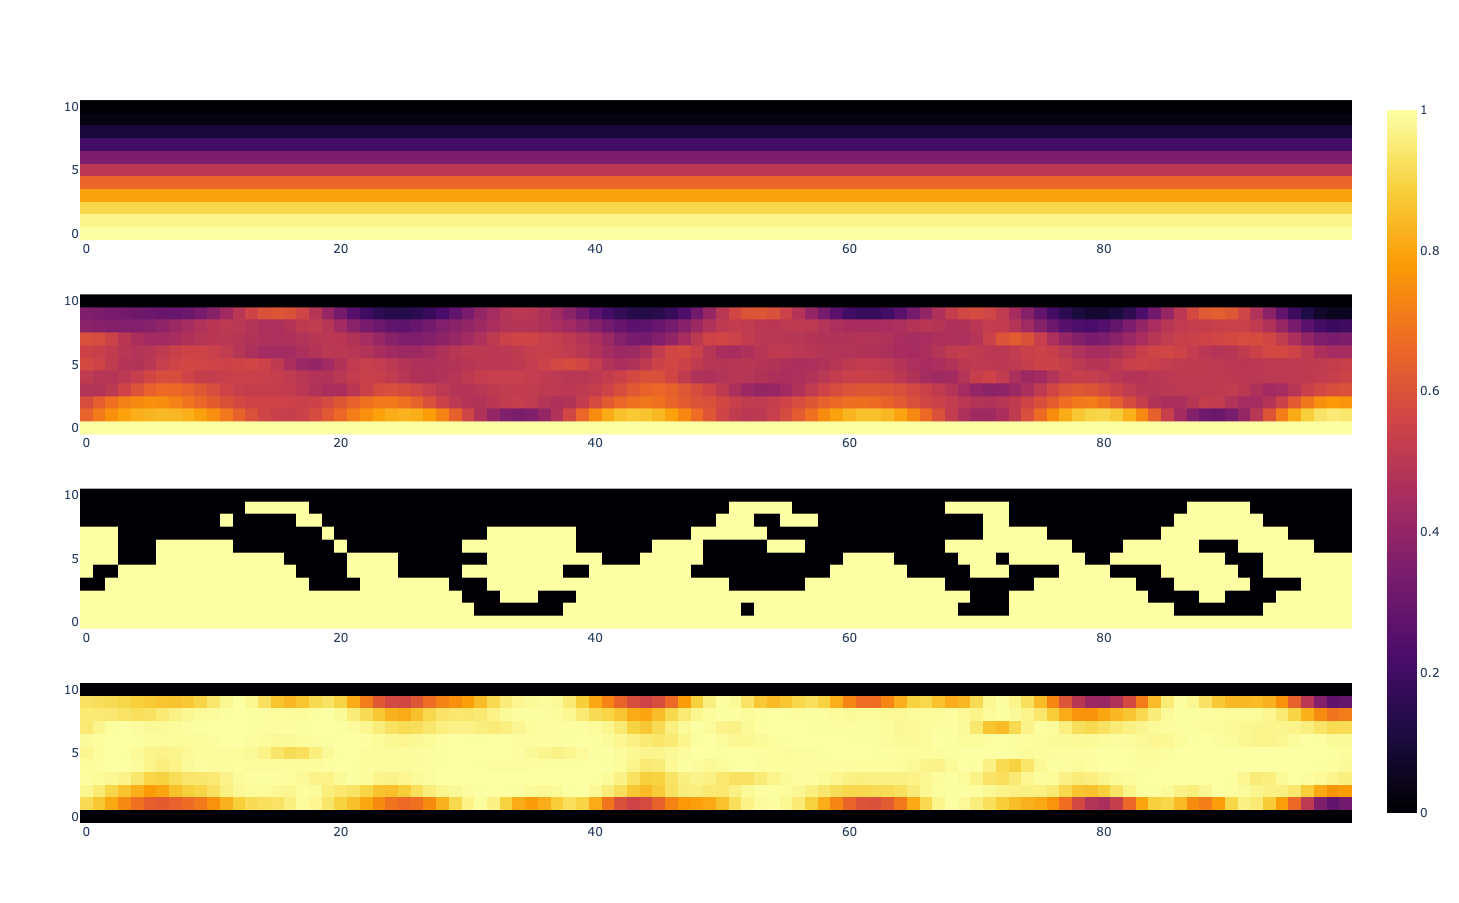
\includegraphics[width=\columnwidth]{graphics/gradient_150_slow_from70_all.png}
    \end{figure}
    }
    \end{columns}
    }
\end{frame}

\end{document}